%%%%%%%%%%%%%%%%%%%%%%%%%%%%%%%%%%%%%%%%%
% Maggi Memoir Thesis
% XeLaTeX Template
% Version 1.0 (22/12/13)
%
% This template has been downloaded from:
% http://www.LaTeXTemplates.com
%
% Original authors:
% Federico Maggi (fede@maggi.cc) with extensive modifications by:
% Vel (vel@latextemplates.com)
%
% License:
% CC BY-NC-SA 3.0 (http://creativecommons.org/licenses/by-nc-sa/3.0/)
%
% Important notes:
% This template needs to be compiled with XeLaTeX.
%
% Most of the document content and packages are specified within structure.tex
% so if you need to make modifications to the template have a look there first!
%
% This template uses several fonts that are not available on most operating 
% systems by default. These are: Adobe Caslon Pro, Envy Code R and 
% Optima Regular. You will either need to obtain these and install them on your
% system or change them to different fonts. Simply go to the Fonts block just
% below here and modify their names to other fonts. You can also comment them 
% out completely to use the default LaTeX font.
%
%%%%%%%%%%%%%%%%%%%%%%%%%%%%%%%%%%%%%%%%%

%----------------------------------------------------------------------------------------
%	PACKAGES AND OTHER DOCUMENT CONFIGURATIONS
%----------------------------------------------------------------------------------------

\documentclass[10pt,showtrims,a4paper,twoside]{memoir} % Change font size here (allowable values are 9pt-12pt), change the paper size, specify one or two sided printing and specify whether to show trimming lines

%----------------------------------------------------------------------------------------
%	VARIOUS REQUIRED PACKAGES AND CONFIGURATIONS
%----------------------------------------------------------------------------------------

\XeTeXinputencoding latin1
\usepackage[T1]{fontenc} % Support for more character glyphs
\usepackage[round]{natbib}\citeindextrue % Round brackets around citations, change to square for square brackets
\usepackage{graphicx} % Required to include images
\usepackage{color} % Required for custom colors
\usepackage{amsmath,amssymb,theorem} % Math packages
\usepackage{listings} % Required for including snippets of code
\usepackage{booktabs} % Required for better horizontal rules in tables
\usepackage{xspace} % Provides the ability to use an intelligent space which is used in \institution and \department
\usepackage[printonlyused,withpage]{acronym} % Include a list of acronyms
\usepackage{rotating} % Allows tables and figures to be rotated
\usepackage{hyperref} % Required for links and changing link options
\usepackage{fontspec} % Required for specifying custom fonts in XeTeX
\usepackage{microtype} % Slightly tweak font spacing for aesthetics

\hypersetup{colorlinks, breaklinks, linkcolor=black,citecolor=black,filecolor=black,urlcolor=black} % Set up hyperlinks including colors for references, urls and citations

%\definecolor{c64}{rgb}{.063,0,.612} % Example color definition, the color can be used with the \color{name} command

\makeatletter
\renewcommand{\fnum@figure}{\textsc{\figurename~\thefigure}} % Make the "Figure 1.1" text in small caps
\makeatother

%----------------------------------------------------------------------------------------
%	PAGE LAYOUT
%----------------------------------------------------------------------------------------

% The memoir class used in this template contains the ability to set the stock paper size and the trimmed size independently. It also has the ability to show trim lines showing where stock paper should be trimmed to get the final book size. This can all be a bit confusing so please see the memoir class documentation for more information.

% By default, the paper size is a4paper which is 29.7cm × 21cm. To change this, simply change "a4paper" in the \documentclass[a4paper,...]{memoir} command in thesis.tex to another size such as "letterpaper".
% By default, the trimmed size is 24cm x 17cm and trim lines are shown. To remove trim lines, simply remove "showtrims" from the \documentclass[showtrims,...]{memoir} command in thesis.tex. The size of the trimmed content is set with the \settrimmedsize{}{} command below.
% If you wish to remove trims and set the content to fit the paper size (i.e. no trimming at all), all you have to do is remove "showtrims" as above and comment out the \settrimmedsize{}{} command below.

%\setstocksize{24cm}{17cm} % Uncomment to manually set the stock size and override the setting in \documentclass
\settrimmedsize{24cm}{17cm}{*} % Change the trimmed area size or comment out this line entirely to fit the content to the paper size without trimming
\setlrmarginsandblock{37.125mm}{*}{0.9} % The first bracket specifies the spine margin, the second the edge margin and the third the ratio of the spine to the edge. Only one or two values are required and the remaining one(s) can be a star (*) to specify it is not needed. By default the edge margin is 10% smaller and 
\setulmarginsandblock{37.125mm}{*}{*} % The first bracket specifies the upper margin, the second the lower margin and the third the ratio of the upper to the lower. Only one or two values are required and the remaining one(s) can be a star (*) to specify it is not needed.
\setmarginnotes{17pt}{51pt}{\onelineskip} % The size of marginal notes, the three values in curly brackets are \marginparsep, \marginparwidth and \marginparpush
\setheadfoot{\onelineskip}{2\onelineskip} % Sets the space available for the header and footer
\setheaderspaces{*}{2\onelineskip}{*} % Sets the spacing above and below the header
\setlength{\trimtop}{0pt} % Sets the spacing above the trimmed area, i.e. moved the trimmed area down the page if positive

% Comment the two lines below to reverse the position of the trimmed content on the stock paper, i.e. odd pages will have content on the right side instead of the left and even pages will have content on the left side instead of the right
\setlength{\trimedge}{\stockwidth}
\addtolength{\trimedge}{-\paperwidth}

\checkandfixthelayout % Makes sure your specifications are correct and implements them in the document

%----------------------------------------------------------------------------------------
%	CHAPTER HEADING STYLE
%----------------------------------------------------------------------------------------

\makeatletter
\makechapterstyle{thesis}{
\renewcommand{\chapternamenum}{}
\setlength{\beforechapskip}{0pt}
\setlength{\midchapskip}{0pt}
\setlength{\afterchapskip}{0pt}
\renewcommand{\chapnamefont}{\LARGE}
\renewcommand{\chapnumfont}{\chapnamefont}
\renewcommand{\chaptitlefont}{\chapnamefont}
\renewcommand{\printchapternum}{}
\renewcommand{\afterchapternum}{}
\renewcommand{\printchaptername}{}
\renewcommand{\afterchaptertitle}{\chapnumfont\hfill\thechapter\\\vspace*{-.3cm}\hrulefill\vspace*{6cm}\\}
}
\makeatother

%----------------------------------------------------------------------------------------
%	TABLE OF CONTENTS DEPTH
%----------------------------------------------------------------------------------------

\maxsecnumdepth{subsubsection}
\maxtocdepth{subsection}

%----------------------------------------------------------------------------------------
%	MATH THEOREM DEFINITIONS
%----------------------------------------------------------------------------------------

\theoremstyle{plain}
\newtheorem{thm}{Theorem}[section] % Defines the theorem environment
\newtheorem{prop}[thm]{Proposition} % Defines the proposition environment
\newtheorem{proof}{Proof}[section] % Defines the proof environment
\newtheorem{definition}{Definition}[section] % Defines the definition environment
\newtheorem{example}{Example}[section] % Defines the example environment
\newtheorem{rem}{Remark} % Defines the remark environment
\newtheorem{note}{Note}[section] % Defines the note environment

%----------------------------------------------------------------------------------------
%	CODE SNIPPET CONFIGURATION
%----------------------------------------------------------------------------------------

\lstset{
  basicstyle=\ttfamily\small,
  basewidth=0.55em,
  showstringspaces=false,
  numbers=left,
  numberstyle=\tiny,
  numbersep=2.5pt,
  keywordstyle=\bfseries\ttfamily,
  breaklines=true
}
% Examples of list environments for different programming languages, you will likely need to specify your own
\lstnewenvironment{pseudoc}{\lstset{frame=lines,language=C,mathescape=true}}{}
\lstnewenvironment{logs}{\lstset{frame=lines,basicstyle=\footnotesize\ttfamily,numbers=none}}{}
\lstnewenvironment{cc}{\lstset{frame=lines,language=C}}{}
\lstnewenvironment{c64}{\lstset{backgroundcolor=\color{c64},basewidth=0.65em,basicstyle=\commodoreface\color{c64light},numbers=none,framerule=10pt,rulecolor=\color{c64light},frame=tb,framexbottommargin=30pt}}{}
\lstnewenvironment{html}{\lstset{frame=lines,language=html,numbers=none}}{}
\lstnewenvironment{pseudo}{\lstset{frame=lines,mathescape=true,morekeywords={learn_string_domain, save_model}}}{}
\lstnewenvironment{pseudoctiny}{\lstset{language=C,mathescape=true,basicstyle=\tiny\sffamily}}{}
\lstnewenvironment{cctiny}{\lstset{language=C,basicstyle=\tiny\sffamily}}{}
\lstnewenvironment{pseudotiny}{\lstset{mathescape=true,basicstyle=\tiny\sffamily}}{} % Include the file containing the code defining the structure and style of the document

%------------------------------------------------
% Thesis Information

\title{Integrated Detection of Anomalous Behavior of Computer Infrastructures} % Thesis title

\author{Federico Maggi} % Author name

\date{December 2013} % The date

\newcommand{\institution}{University of California\xspace} % University/institution name

\newcommand{\department}{Department of Computer Science\xspace} % Department name

%------------------------------------------------
% Fonts

\defaultfontfeatures{Mapping=tex-text}
\setromanfont[Ligatures={Common}]{Adobe Caslon Pro} % Normal document font
\setmonofont[Scale=0.8]{Envy Code R} % Mono spaced font (\texttt{})
\setsansfont[Scale=0.9]{Optima Regular} % Sans-serif font (\textsf{})

\renewcommand*{\acffont}[1]{{\normalsize\itshape #1}} % Font style for the acronym text (e.g. Do It Yourself)
\renewcommand*{\acfsfont}[1]{{\normalsize\upshape #1}} % Font style for the acronym in bracket (e.g. (DIY))

%------------------------------------------------
% Hyphenations

\hyphenation{a-no-ma-lous a-no-ma-ly amounts breaches} % Specify custom hyphenation points in words with dashes where you would like hyphenation to occur, or alternatively, don't put any dashes in a word to stop hyphenation altogether

%----------------------------------------------------------------------------------------
%	TITLE PAGE
%----------------------------------------------------------------------------------------

\renewcommand{\maketitlehooka}{
\centering

\includegraphics[width=2.5cm]{Figures/polimi-logo}\\[.5cm] % Institution logo
\institution\\ % Print institution name
\emph{\department}\\[.2cm] % Print department name
DOTTORATO DI RICERCA IN INGEGNERIA DELL'INFORMAZIONE % Degree or other information
\par
\hrulefill
\vfill}
\renewcommand{\maketitlehookb}{\vfill}
\renewcommand{\maketitlehookc}{
\vfill
\begin{flushleft}
Advisor:\\
\textbf{Prof. Stefano Zanero}\\[.3cm] % Advisor's/supervisor's name
Tutor:\\
\textbf{Prof. Letizia Tanca}\\[.3cm] % Tutor's name
Supervisor of the Doctoral Program:\\
\textbf{Prof. Patrizio Colaneri} % Doctoral program supervisor's name
\end{flushleft}
\vfill}
\preauthor{\begin{flushright}Doctoral Dissertation of:\\\bfseries} % Text prior to the author name - right aligned and bold
\postauthor{\end{flushright}} % After the author name, stop right alignment

%----------------------------------------------------------------------------------------

\makeindex % Write an index file

\begin{document}

\begin{titlingpage}
\maketitle % Print the title page
\end{titlingpage}

\frontmatter % Use roman page numbering style (i, ii, iii, iv...) for the pre-content pages

%----------------------------------------------------------------------------------------
%	PREFACE
%----------------------------------------------------------------------------------------

\section*{Preface}
This thesis embraces all the efforts that I put during the last three years as a PhD student at Politecnico di Milano. I have been working under the supervision of Prof. S. Zanero and Prof. G. Serazzi, who is also the leader of the research group I am part of. In this time frame I had the wonderful opportunity of being ``initiated'' to research, which radically changed the way I look at things: I found my natural \emph{``thinking outside the box''} attitude --- that was probably well-hidden under a thick layer of lack-of-opportunities, I took part of very interesting joint works --- among which the year I spent at the Computer Security Laboratory at UC Santa Barbara is at the first place, and I discovered the Zen of my life.

My research is all about \emph{computers} and every other technology possibly related to them. Clearly, the way I look at computers has changed a bit since when I was seven. Still, I can remember me, typing on that \textsf{Commodore} 64 in front of a tube TV screen, trying to get that d---n routine written in \textsf{Basic} to work. I was just playing, obviously, but when I recently found a picture of me in front of that screen...it all became clear.

So, although my attempt of writing a program to authenticate myself was a little bit naive --- being limited to a print instruction up to that point apart, of course --- I thought \emph{``maybe I am not in the wrong place, and the fact that my research is still about security is a good sign''}!

Many years later, this work comes to life. There is a humongous amount of people that, directly or indirectly, have contributed to my research and, in particular, to this work. Since my first step into the lab, I will not, ever, be thankful enough to Stefano, who, despite my skepticism, convinced me to submit that application for the PhD program. For trusting me since the very first moment I am thankful to Prof. G. Serazzi as well, who has been always supportive. For hosting and supporting my research abroad I thank Prof. G. Vigna, Prof. C. Kruegel, and Prof. R. Kemmerer. Also, I wish to thank Prof. M. Matteucci for the great collaboration, Prof. I. Epifani for her insightful suggestions and Prof. H. Bos for the detailed review and the constructive comments.

On the colleagues-side of this acknowledgments I put all the fellows of Room 157, Guido, the crew of the seclab and, in particular, Wil with whom I shared all the pain of paper writing between Sept '08 and Jun '09.

On the friends-side of this list Lorenzo and Simona go first, for being our family.

I have tried to translate in simple words the infinite gratitude I have and will always have to Valentina and my parents for being my fixed point in my life. Obviously, I failed.

\begin{flushright}
\textsc{\theauthor}\\
Milano\\
September 2009
\end{flushright}

\cleartoverso % Force a break to an even page

%----------------------------------------------------------------------------------------
%	ABSTRACT
%----------------------------------------------------------------------------------------

\begin{abstract}
This dissertation details our research on anomaly detection techniques, that are central to several classic security-related tasks such as network monitoring, but it also have broader applications such as program behavior characterization or malware\index{malware} classification. In particular, we worked on anomaly detection from three different perspective, with the common goal of recognizing awkward activity on computer infrastructures. In fact, a computer system has several weak spots that must be protected to avoid attackers to take advantage of them. We focused on protecting the operating system, central to any computer, to avoid malicious code to subvert its normal activity. Secondly, we concentrated on protecting the web applications, which can be considered the modern, shared operating systems; because of their immense popularity, they have indeed become the most targeted entry point to violate a system. Last, we experimented with novel techniques with the aim of identifying related events (e.g., alerts reported by intrusion detection systems) to build new and more compact knowledge to detect malicious activity on large-scale systems.

Our contributions regarding host-based protection systems focus on characterizing a process' behavior through the system calls invoked into the kernel. In particular, we engineered and carefully tested different versions of a multi-model detection system using both stochastic and deterministic models to capture the features of the system calls during normal operation of the operating system. Besides demonstrating the effectiveness of our approaches, we confirmed that the use of finite-state, deterministic models allow to detect deviations from the process' control flow with the highest accuracy; however, our contribution combine this effectiveness with advanced models for the system calls' arguments resulting in a significantly decreased number of false alarms.

Our contributions regarding web-based protection systems focus on advanced training procedures to enable learning systems to perform well even in presence of changes in the web application source code --- particularly frequent in the Web 2.0 era. We also addressed data scarcity issues that is a real problem when deploying an anomaly detector to protect a new, never-used-before application. Both these issues dramatically decrease the detection capabilities of an intrusion detection system but can be effectively mitigated by adopting the techniques we propose.

Last, we investigated the use of different stochastic and fuzzy models to perform automatic alert correlation, which is as post processing step to intrusion detection. We proposed a fuzzy model that formally defines the errors that inevitably occur if time-based alert aggregation (i.e., two alerts are considered correlated if they are close in time) is used. This model allow to account for measurements errors and avoid false correlations due to delays, for instance, or incorrect parameter settings. In addition, we defined a model to describe the alert generation as a stochastic process and experimented with non-parametric statistical tests to define robust, zero-configuration correlation systems.

The aforementioned tools have been tested over different datasets --- that are thoroughly documented in this document --- and lead to interesting results.
\end{abstract}

\cleartoverso % Force a break to an even page

%----------------------------------------------------------------------------------------
%	TABLE OF CONTENTS
%----------------------------------------------------------------------------------------

\tableofcontents* % Print the table of contents

\cleartoverso % Force a break to an even page

%----------------------------------------------------------------------------------------
%	LIST OF FIGURES
%----------------------------------------------------------------------------------------

\listoffigures % Print the list of figures

\cleartoverso % Force a break to an even page

%----------------------------------------------------------------------------------------
%	LIST OF TABLES
%----------------------------------------------------------------------------------------

\listoftables % Print the list of tables

\cleartoverso % Force a break to an even page

%----------------------------------------------------------------------------------------
%	ACRONYMS
%----------------------------------------------------------------------------------------

\chapter{List of Acronyms}
\begin{acronym}\addtolength{\itemsep}{-\baselineskip}
  \acro{AIC}{Akaike Information Criterion}
  \acro{ARMA}{Auto Regressive Moving Average}
  \acro{ARMAX}{Auto Regressive Moving Average eXogenous}
  \acro{ARX}{Auto Regressive eXogenous}
  \acro{AR}{Auto Regressive}
  \acro{ARR}{Alert Reduction Rate}
  \acro{ANSI}{American National Standard Institute}
  \acro{ASCII}{American Standard for Information Interxchange}
  \acro{BIC}{Bayesian Information Criterion}
  \acro{BMU}{Best Matching Unit}
  \acro{BSM}{Basic Security Module}
  \acro{CDF}{Cumulative Density Function}
  \acro{CDX}{Cyber Defense eXercise}
  \acro{CIA}{Confidentially Integrity Availability}
  \acro{CIDS}{Collaborative IDS}
  \acro{CPU}{Central Processing Unit}
  \acro{CSV}{Comma Separated Values}
  \acro{CTF}{Capture The Flag}
  \acro{DAG}{Direct Acyclic Graph}
  \acro{DARPA}{Defense Advanced Research Projects Agency}
  \acro{DB}{DataBase}
  \acro{DBMS}{DataBase Management System}
  \acro{DIDS}{Distributed IDS}
  \acro{DNS}{Domain Name System}
  \acro{DOM}{Document Object Model}
  \acro{DoS}{Denial of Service}
  \acro{DR}{Detection Rate}
  \acro{DTD}{Document Type Definition}
  \acro{ED}{Elementary Detector}
  \acro{ELF}{Executable Linux Format}
  \acro{FN}{False Negative}
  \acro{FNR}{False Negative Rate}
  \acro{FPR}{False Positive Rate}
  \acro{FP}{False Positive}
  \acro{FSA}{Finite State Automaton}
  \acro{FTP}{File Transfer Protocol}
  \acro{GCI}{Granger Causality Index}
  \acro{GCT}{Granger Causality Test}
  \acro{HIDS}{Host-based Intrusion Detection System}
  \acro{HMM}{Hidden Markov Model}
  \acro{HTML}{HyperText Markup Language}
  \acro{HTTP}{HyperText Transfer Protocol}
  \acro{ICD}{Idealized Character Distribution}
  \acro{IDEVAL}{Intrusion Detection eVALuation}
  \acro{IDMEF}{Intrusion Detection Message Exchange Format}
  \acro{IDS}{Intrusion Detection System}
  \acro{IDWG}{Intrusion Detection Working Group}
  \acro{ID}{Intrusion Detection}
  \acro{IETF}{Internet Engineering Task Force}
  \acro{IODEF}{Incident Object Description and Interchange Format}
  \acro{IPS}{Intrusion Protection System}
  \acro{ISP}{Internet Service Provider}
  \acro{IP}{Internet Protocol}
  \acro{IR}{Information Retrieval}
  \acro{IRC}{Internet Relay Chat}
  \acro{ISS}{Internet Security Systems}
  \acro{JSON}{JavaScript Object Notation}
  \acro{KBS}{Knowledge Base System}
  \acro{KS}{Kolmogorov-Smirnoff}
  \acro{LARIAT}{Lincoln Adaptable Real-time Information Assurance Testbed}
  \acro{LERAD}{Learning Rules for Anomaly Detection}
  \acro{LL}{Lincoln Laboratory}
  \acro{MDL}{Minimum Description Length}
  \acro{MIT}{Massachusetts Institute of Technology}
  \acro{ML}{Maximum Likelihood}
  \acro{MTU}{Maximum Transfer Unit}
  \acro{NIDES}{Next-generation Intrusion Detection Expert System}
  \acro{NIDS}{Network-based Intrusion Detection System}
  \acro{NNID}{Neural Network Intrusion Detection}
  \acro{NSTISSC}{National Security Telecomm. and Information Systems Sec. Committee}
  \acro{NTP}{Network Time Protocol}
  \acro{PC}{Program Counter}
  \acro{PDF}{Probability Density Function}
  \acro{PHAD}{Packet Header Anomaly Detection}
  \acro{PHP}{PHP Hypertext Preprocessor}
  \acro{PID}{Process IDentifier}
  \acro{ROC}{Receiving Operating Characteristic}
  \acro{SADE}{Syscall Sequence Arguments Anomaly Detection Engine}
  \acro{SDEE}{Security Device Event Exchange}
  \acro{SMTP}{Simple Message Transfer Protocol}
  \acro{SOM}{Self Organizing Map}
  \acro{SQL}{Structured Query Language}  
  \acro{SRI}{Stanford Research Institute}
  \acro{SSH}{Secure SHell}
  \acro{STATL}{State Transition Analysis Technique Language}
  \acro{SVN}{SubVersioN}
  \acro{SYN}{SYNchronize}
  \acro{TCP}{Trasmission Control Protocol}
  \acro{TF}{Truth File}
  \acro{TN}{True Negative}
  \acro{TNR}{True Negative Rate}
  \acro{TOS}{Type Of Service}
  \acro{TP}{True Positive}
  \acro{TTL}{Time To Live}
  \acro{UCSB}{University of California Santa Barbara}
  \acro{ULISSE}{Unsupervised Learning IDS with 2-Stages Engine}
  \acro{UDP}{User Datagram Protocol}
  \acro{UML}{Unified Modeling Language}
  \acro{URL}{Uniform Resource Locator}
  \acro{VPN}{Virtual Private Network}
  \acro{XML}{eXtensible Markup Language}
  \acro{XSD}{XML Schema Definition}
  \acro{XSS}{Cross-Site Scripting}
\end{acronym} % Include a List of Acronyms section using acronyms.tex where they are defined

\cleartoverso % Force a break to an even page

%----------------------------------------------------------------------------------------
%	COLOPHON
%----------------------------------------------------------------------------------------

\thispagestyle{empty} % Remove all headers and footers from this page

\vspace*{2em}
\renewcommand{\abstractname}{Colophon}
\begin{abstract}
This document was typeset using the \textsf{XeTeX} typesetting system created by the Non-Roman Script Initiative and the memoir class created by Peter Wilson. The body text is set 10pt with~Adobe Caslon Pro. Other fonts include \texttt{Envy Code R}, \textsf{Optima Regular} and. Most of the drawings are typeset using the \textsf{TikZ/PGF} packages by Till Tantau.
\end{abstract}
\vfill

%----------------------------------------------------------------------------------------
%	CONTENT CHAPTERS
%----------------------------------------------------------------------------------------

\mainmatter % Begin numeric (1,2,3...) page numbering

\chapterstyle{thesis} % Change the style of the Chapter header to that defined in structure.tex

\pagestyle{Ruled} % Include the chapter/section in the header along with a horizontal rule underneath

\chapter{Introduction}
\label{introduction}

Network connected devices such as personal computers, mobile phones, or gaming consoles are nowadays enjoying immense popularity. In parallel, the Web and the humongous amount of services it offers have certainly became the most ubiquitous tools of all the times. \textsf{Facebook} counts more than 250 millions active users of which 65 millions are using it on mobile devices; not to mention that more than 1 billion photos are uploaded to the site \emph{each   month}~\citep{facebook-stats}. And this is just one, popular website. One year ago, \textsf{Google} estimated that the approximate number of unique \acp{URL}\index{URL} is 1 trillion~\citep{google-is-big}, while \texttt{YouTube} has stocked more than 70 million videos as of March 2008, with 112,486,327 views just on the most popular video as of January 2009~\citep{social-media-stats}. And people from all over the world inundate the Web with more than 3 million tweets \emph{per day}. Not only the Web 2.0 has became predominant; in fact, thinking that on December 1990 the Internet was made of \emph{one} site and today it counts more than 100 million sites is just astonishing~\citep{internet-timeline}.

The Internet and the Web are huge~\citep{inetworldstats}. The relevant fact, however, is that they both became the most advanced workplace. Almost every industry connected its own network to the Internet and relies on these infrastructures for a vast majority of transactions; most of the time monetary transactions. As an example, every year \textsf{Google} looses approximately 110 millions of US Dollars in ignored ads because of the \emph{``I'm feeling lucky''} button. The scary part is that, during their daily work activities, people typically pay poor or no attention at all to the risks that derive from exchanging any kind of information over such a complex, interconnected infrastructure. This is demonstrated by the effectiveness of social engineering~\citep{deception} scams carried over the Internet or the phone~\citep{social-engineering-fundamentals}. Recall that 76\% of the phishing is related to finance. Now, compare this landscape to what the most famous security quote states.

\begin{quotation}
  ``The only truly secure computer is one buried in concrete, with the   power turned off and the network cable cut''.
   ---\emph{Anonymous}
\end{quotation}

In fact, the Internet is all but a safe place~\citep{whid}, with more than 1,250 \emph{known} data breaches between 2005 and 2009 \citep{data-breaches-chronology} and an estimate of 263,470,869 records stolen by intruders. One may wonder why the advance of research in computer security and the increased awareness of governments and public institutions are still not capable of avoiding such incidents. Besides the fact that the aforementioned numbers would be order of magnitude higher in absence of countermeasures, todays' security issues are, basically, caused by the combination of two phenomena: the high amount of software vulnerabilities and the effectiveness of todays' exploitation strategy.

\begin{description}
\item[software flaws] --- (un)surprisingly, software is affected by   vulnerabilities. Incidentally, tools that have to do with the Web,   namely, browsers and 3\textsuperscript{rd}-party extensions, and web   applications, are the most vulnerable ones. For instance, in 2008,   \textsf{Secunia} reported around 115 security vulnerabilities for   \textsf{Mozilla Firefox}, 366 for \textsf{Internet Explorer}'s   \textsf{ActiveX}~\citep{secunia2008}. Office suites and e-mail   clients, that are certainly the must-have-installed tool   on every workstation, hold the second position~\citep{sans20}.
  
\item[massification of attacks] --- in parallel to the explosion of   the Web 2.0, attackers and the underground economy have quickly   learned that a sweep of exploits run against \emph{every} reachable   host have more chances to find a vulnerable target and, thus, is   much more profitable compared to a single effort to break into a   high-value, well-protected machine.
\end{description}

These circumstances have initiated a vicious circle that provides the attackers with a very large pool of vulnerable targets. Vulnerable client hosts are compromised to ensure virtually unlimited bandwidth and computational resources to attackers, while server side applications are violated to host malicious code used to infect client visitors. And so forth. An old fashioned attacker would have violated a single site using all the resources available, stolen data and sold it to the underground market. Instead, a modern attacker adopts a ``vampire'' approach and exploit client-side software vulnerabilities to take (remote) control of million hosts. In the past the diffusion of malicious code such as viruses was sustained by sharing of infected, cracked software through floppy or compact disks; nowadays, the Web offers unlimited, public storage to attackers that deploy their exploit on compromised websites.

Thus, not only the type of vulnerabilities has changed, posing virtually every interconnected device at risk. The exploitation strategy created new types of threats that take advantage of classic malicious code patterns but in a new, extensive, and tremendously effective way.

\section{Todays' Security Threats}
\label{introduction:motivation} Every year, new threats are discovered and attacker take advantage of them until effective countermeasures are found. Then, new threats are discovered, and so forth. \textsf{Symantec} quantifies the amount of new malicious code threats to be 1,656,227 as of 2008 \citep{symantec_threat_report_2009}, 624,267 one year earlier and only 20,547 in 2002. Thus, countermeasures must advance at least with the same grow rate. In addition:

\begin{figure}[t]
  \centering
  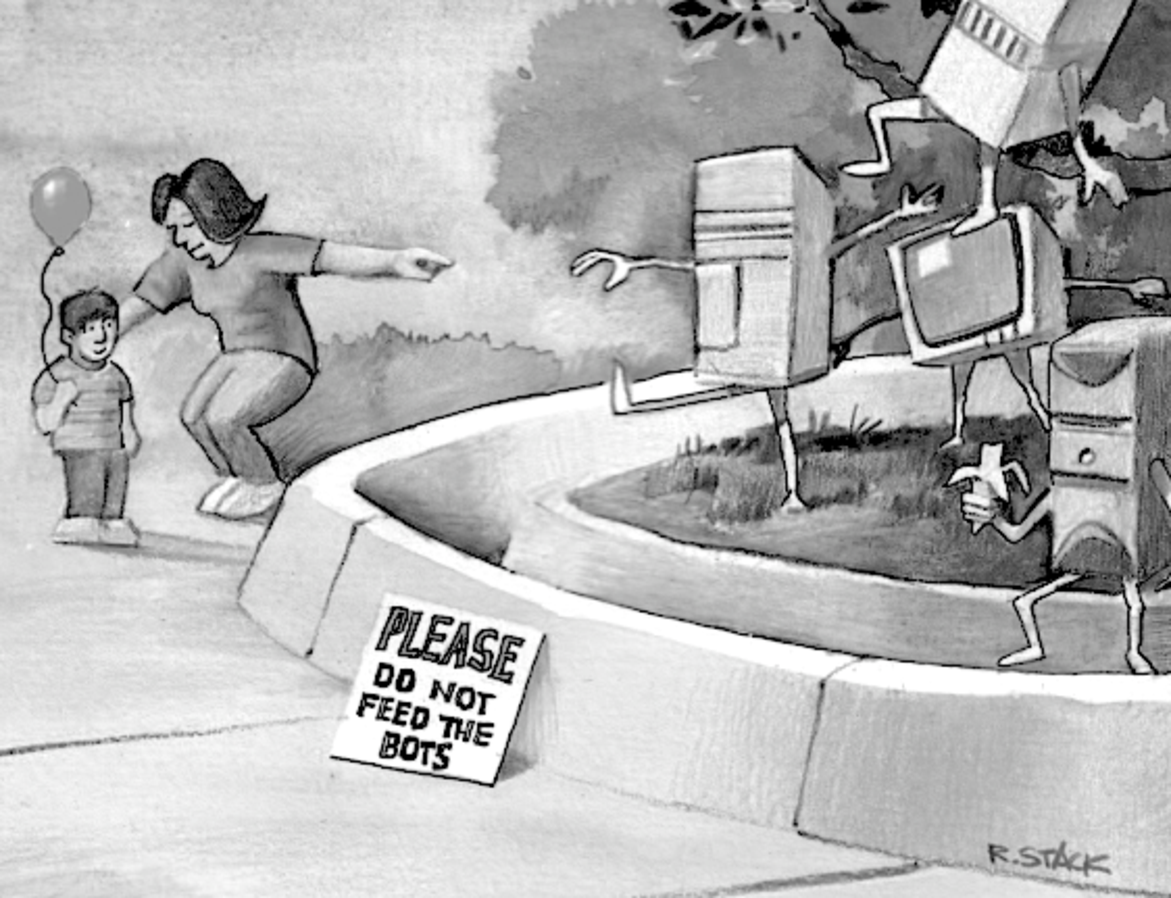
\includegraphics[width=\textwidth]{Figures/bots.pdf}
  \caption{Illustration taken from~\citep{holz} and \copyright 2005 IEEE. Authorized license limited to \institution.}
  \label{fig:bots}
\end{figure}

\begin{quotation}
  [...] the current threat landscape --- such as the increasing complexity and sophistication of attacks, the evolution of attackers
and attack patterns, and malicious activities being pushed to emerging countries --- show not just the benefits of, but also the need for increased cooperation among security companies, governments, academics, and other organizations and individuals to combat these changes~\citep{symantec_threat_report_2009}.
\end{quotation}

Todays' underground economy run a very proficient market: everyone can buy credit card information for as low as \$0.06--\$30, full identities for just \$0.70--\$60 or rent a scam hosting solution for \$3--\$40 per week plus \$2-\$20 for the design~\citep{symantec_threat_report_2009}.

The main underlying technology actually employs a classic type of software called \emph{bot} (jargon for \emph{robot}), which is not malicious \emph{per s\'e}, but is used to remotely control a network of compromised hosts, called \emph{botnet}~\citep{holz}. Remote commands can be of any type and typically include launching an attack, starting a phishing or spam campaign, or even updating to the latest version of the bot software by downloading the binary code from a host controlled by the attackers (usually called \emph{bot master})~\citep{torpig}. The exchange good has now become the botnet infrastructure itself rather than the data that can be stolen or the spam that can be sent. These are mere outputs of todays' most popular service offered for rent by the underground economy.

\subsection{The Role of Intrusion Detection}
\label{introduction:motivation:ids-role}
The aforementioned, dramatic big picture may lead to think that the malicious software will eventually proliferate at every host of the Internet and no effective remediation exists. However, a more careful analysis reveals that, despite the complexity of this scenario, the problems that must be solved by a security infrastructure can be decomposed into relatively simple tasks that, surprisingly, may already have a solution. Let us look at an example.

\begin{example}
This is how a sample exploitation can be structured:
\begin{description}
\item [injection] --- a malicious request is sent to the vulnerable web application with the goal of corrupting all the responses sent to legitimate clients from that moment on. For instance, more than one releases of the popular \textsf{WordPress} blog application are vulnerable to injection attacks\footnote{http://secunia.com/advisories/23595} that allow an attacker to permanently include arbitrary content to the pages. Typically, such an arbitrary content is malicious code (e.g., JavaScript, VBSCrip, ActionScript, ActiveX) that, every time a legitimate user requests the infected page, executes on the client host.
\item [infection] --- Assuming that the compromised site is frequently accessed --- this might be the realistic case of the \textsf{WordPress}-powered \textsf{ZDNet} news blog\footnote{http://wordpress.org/showcase/zdnet/} --- a significant amount of clients visit it. Due to the high popularity of vulnerable browsers and plug-ins, the client may run \textsf{Internet Explorer} --- that is the most popular --- or an outdated release of \textsf{Firefox} on \textsf{Windows}. This create the perfect circumstances for the malicious page to successfully execute. In the best case, it may download a virus or a generic malware from a website under control of the attacker, so infecting the machine. In the worst case, this code may also exploit specific browser vulnerabilities and execute in privileged mode.
\item [control \& use] --- The malicious code just download installs and hides itself onto the victim's computer, which has just joined a botnet. As part of it, the client host can be remotely controlled by the attackers who can, for instance, rent it, use its bandwidth and computational power along with other computers to run a distributed \ac{DoS} attack. Also, the host can be used to automatically perform the same attacks described above against other vulnerable web applications. And so forth. \end{description}
\end{example}

This simple yet quite realistic example shows the various kinds of malicious activity that are generated during a typical drive-by exploitation. It also shows its requirements and assumptions that must hold to guarantee success. More precisely, we can recognize:

\begin{description}
\item[network activity] --- clearly, the whole interaction relies on a network connection over the Internet: the \ac{HTTP} connections used, for instance, to download the malicious code as well as to launch the injection attack used to compromise the web server.
\item[host activity] --- similarly to every other type of attack against an application, when the client-side code executes, the browser (or one of its extension plug-ins) is forced to behave improperly. If the malicious code executes till completion the attack succeeds and the host is infected. This happens only if the platform, operating system, and browser all match the requirements assumed by the exploit designer. For instance, the attack may succeed on \textsf{Windows} and not on \textsf{Mac OS X}, although the vulnerable version of, say, \textsf{Firefox} is the same on both the hosts.
\item[HTTP traffic] --- in order to exploit the vulnerability of the web application, the attacking client must generate malicious \ac{HTTP} requests. For instance, in the case of an \ac{SQL} injection --- that is the second most common vulnerability in a web application --- instead of a regular

\begin{logs}
GET /index.php?username=myuser
\end{logs}
  
\noindent the web server might be forced to process a

\begin{logs}
GET /index.php?username=' OR 'x'='x'--\&content=<script src="evil.com/code.js">
\end{logs}

\noindent that causes the \texttt{index.php} page to behave improperly.
\end{description}

It is now clear that protection mechanisms that analyze the network traffic, the activity of the client's operating system, the web server's \ac{HTTP} logs, or any combination of the three, have chances of recognizing that something malicious is happening in the network. For instance, if the \ac{ISP} network adopt \textsf{Snort}, a lightweight \ac{IDS} that analyzes the network traffic for known attack patterns, could block all the packets marked as suspicious. This would prevent, for instance, the \ac{SQL} injection to reach the web application. A similar protection level can be achieved by using other tools such as \textsf{ModSecurity} \citep{ristic:mod_security}. One of the problems that may arise with these classic, widely adopted solutions is if a zero day\index{0-day} attack is used. A zero day attack or threat exploits a vulnerability that is unknown to the public, undisclosed to the software vendor, or a fix is not available; thus, protection mechanisms that merely blacklist known malicious activity immediately become ineffective. In a similar vein, if the client is protected by an anti-virus, the infection phase can be blocked. However, this countermeasure is once again successful only if the anti-virus is capable of recognizing the malicious code, which assumes that the code is known to be malicious.

Ideally, an effective and comprehensive countermeasure can be achieved if all the protection tools involved (e.g., client-side, server-side, network-side) can collaborate together. For instance, if a website is publicly reported to be malicious, a client-side protection tool should block all the content downloaded from that particular website. This is only a simple example.

Thus, countermeasures against todays' threats already exist but are subject to at least two drawbacks:

\begin{itemize}
\item they offer protection only against known threats. To be effective we must assume that all the hostile traffic can be enumerated, which is clearly an impossible task.

\begin{quotation}
Why is ``Enumerating Badness'' a dumb idea? It's a dumb idea because sometime around 1992 the amount of Badness in the Internet began to vastly outweigh the amount of Goodness. For every harmless, legitimate, application, there are dozens or hundreds of pieces of malware, worm tests, exploits, or viral code. Examine a typical antivirus package and you'll see it knows about 75,000+ viruses that might infect your machine. Compare that to the legitimate 30 or so apps that I've installed on my machine, and you can see it's rather dumb to try to track 75,000 pieces of Badness when even a simpleton could track 30 pieces of Goodness~\citep{ranum-myths}.
\end{quotation}

\item they lack of cooperation, which is crucial to detect global and slow attacks.
\end{itemize}

This said, we conclude that classic approaches such as dynamic and static code analysis and \ac{IDS} already offer good protection but industry and research should move toward methods that require little or no knowledge. In this work, we indeed focus on the so called anomaly-based approaches, i.e., those that attempt to recognize the threats by detecting any variation from a system's normal operation, rather than looking for signs of known-to-be-malicious activity.

\section{Original Contributions}
\label{introduction:contributions} Our main research area is \ac{ID}. In particular, we focus on anomaly-based approaches to detect malicious activities. Since todays' threats are complex, a single point of inspection is not effective. A more comprehensive monitoring system is more desirable to protect both the network, the applications running on a certain host, and the web applications (that are particularly exposed due to the immense popularity of the Web). Our contributions focus on the mitigation of both host-based and web-based attacks, along with two techniques to correlate alerts from hybrid sensors.

\subsection{Host-based Anomaly Detection} Typical malicious processes can be detected by modeling the characteristics (e.g., type of arguments, sequences) of the system calls executed by the kernel, and by flagging unexpected deviations as attacks. Regarding this type of approaches, our contributions focus on hybrid models to accurately characterize the behavior of a binary application. In particular:

\begin{itemize}
\item we enhanced, re-engineered, and evaluated a novel tool for modeling the normal activity of the Linux 2.6 kernel. Compared to other existing solutions, our system shows better detection capabilities and good contextualization of the alerts reported.
\item We engineered and evaluated an \ac{IDS} to demonstrate that the combined use of (1) deterministic models to characterize a process' control flow and (2) stochastic models to capture normal features of the data flow, lead to better detection accuracy. Compared to the existing deterministic and stochastic approaches separately, our system shows better accuracy, with almost zero false positives.
\item We adapted our techniques for forensics investigation. By running experiments on real-world data and attacks, we show that our system is able to detect hidden tamper evidence although sophisticated anti-forensics tools (e.g., userland process execution) have been used.
\end{itemize}

\subsection{Web-based Anomaly Detection} Attempts of compromising a web application can be detected by modeling the characteristics (e.g., parameter values, character distributions, session content) of the \ac{HTTP}\index{HTTP} messages exchanged between servers and clients during normal operation. This approach can detect virtually any attempt of tampering with \ac{HTTP}\index{HTTP} messages, which is assumed to be evidence of attack. In this research field, our contributions focus on training data scarcity issues along with the problems that arise when an application changes its legit behavior. In particular:

\begin{itemize}
\item we contributed to the development of a system that learns the legit behavior of a web application. Such a behavior is defined by means of features extracted from 1) HTTP requests, 2) HTTP responses, 3) SQL queries to the underlying database, if any. Each feature is extracted and learned by using different models, some of which are improvements over well-known approaches and some others are original. The main contribution of this work is the \emph{combination} of database query models with HTTP-based models. The resulting system has been validated through preliminary experiments that shown very high accuracy.
\item we developed a technique to automatically detect legit changes in web applications with the goal of suppressing the large amount of false detections due to code upgrades, frequent in todays' web applications. We run experiments on real-world data to show that our simple but very effective approach accurately predict changes in web applications and can distinguish good \emph{vs.} malicious changes (i.e., attacks).
\item We designed and evaluated a machine learning technique to aggregate \ac{IDS} models with the goal of ensuring good detection accuracy even in case of scarce training data available. Our approach relies on clustering techniques and nearest-neighbor search to look-up well-trained models used to replace under-trained ones that are prone to overfitting and thus false detections. Experiments on real-world data have shown that almost every false alert due to overfitting is avoided with as low as 32-64 training samples per model.
\end{itemize}

Although these techniques have been developed on top of a web-based anomaly detector, they are sufficiently generic to be easily adapted to other systems using learning approaches.

\subsection{Alert Correlation} \ac{IDS} alerts are usually post-processed to generate compact reports and eliminate redundant, meaningless, or false detections. In this research field, our contributions focus on unsupervised techniques applied to aggregate and correlate alert events with the goal of reducing the effort of the security officer. In particular:

\begin{itemize}
\item We developed and tested an approach that accounts for the common measurement errors (e.g., delays and uncertainties) that occur in the alert generation process. Our approach exploits fuzzy metrics both to model errors and to construct an alert aggregation criterion based on distance in time. This technique has been show to be more robust compared to classic time-distance based aggregation metrics.
\item We designed and tested a prototype that models the alert generation process as a stochastic process. This setting allowed us to construct a simple, non-parametric hypothesis test that can detect whether two alert streams are correlated or not. Besides its simplicity, the advantage of our approach is to not requiring any parameter.
\end{itemize}

The aforementioned results have been published in the proceedings of international conferences and international journals. % Include the introduction chapter
\chapter{A Chapter of Examples}
\label{chapter1}

\section{A Table}

\begin{table}[h]
\centering
\begin{tabular}{rcc}
\toprule \emph{Feature} & \textsc{Misuse-based} &
\textsc{Anomaly-based}\\
    
\midrule Modeled activity: & Malicious & Normal\\
Detection method: & Matching & Deviation\\
Threats detected: & Known & Any\\
False negatives: & High & Low\\
False positives: & Low & High\\
Maintenance cost: & High & Low\\
Attack desc.: & Accurate & Absent\\
System design: & Easy & Difficult\\
\bottomrule
\end{tabular}
\caption[Duality between misuse- and anomaly-based intrusion detection techniques.]{Duality between misuse- and anomaly-based intrusion detection techniques. Note that, an anomaly-based \ac{IDS} can detect ``Any'' threat, under the assumption that an attack always generates a deviation in the modeled activity.}
\label{tab:misuse-vs-anomaly}
\end{table}

%------------------------------------------------

\section{Code}

\begin{pseudoc}
  /* ... */ cd['<'] = {0.1, 0.11} cd['a'] = {0.01, 0.2} cd['b'] =
  {0.13, 0.23} /* ... */

  b = decode(arg3_value);
  
  if ( !(cd['c'][0] < count('c', b) < cd['c'][1]) ||\
       !(cd['<'][0] < count('<', b) < cd['<'][1]) ||\
       ... || ...)  fire_alert("Anomalous content detected!");
  /* ... */
\end{pseudoc}

%------------------------------------------------

\section{A Sideways Table}

\clearpage
\begin{sidewaystable}
\renewcommand{\arraystretch}{1.5} \centering
\begin{tabular}{rcccccc}
\toprule \textsc{Approach} & \textsc{Time} & \textsc{Header} &
\textsc{Payload} & \textsc{Stochastic} & \textsc{Determ.} & \textsc{Clustering}\\
\midrule \citep{phad} & & $\bullet$ & & & & $\bullet$ \\
\citep{kruegel:sac2002:anomaly} & & $\bullet$ & $\bullet$ & $\bullet$ & & \\
\citep{protocolanom} & & $\bullet$ & & $\bullet$ & $\bullet$ & \\
\citep{ramadas} & & & $\bullet$ & & & $\bullet$ \\
\citep{rules-payl} & $\bullet$ & & $\bullet$ & & $\bullet$ & \\
\citep{zanero-savaresi} & & $\bullet$ & $\bullet$ & & & $\bullet$ \\
\citep{wang:raid2004:payl} & & & $\bullet$ & $\bullet$ & & \\
\citep{zanero-pattern} & & $\bullet$ & $\bullet$ & & & $\bullet$ \\
\citep{DBLP:conf/iwia/BolzoniEHZ06} & & $\bullet$ & $\bullet$ & & & $\bullet$ \\
\citep{wang:raid2006:anagram} & & & $\bullet$ & $\bullet$ & & \\
\bottomrule
\end{tabular}
\caption{Taxonomy of the selected state of the art approaches for network-based anomaly detection.}
\label{tab:network-sota-taxonomy}
\end{sidewaystable}
\clearpage

%------------------------------------------------

\section{A Figure}

\begin{figure}[h]
\centering
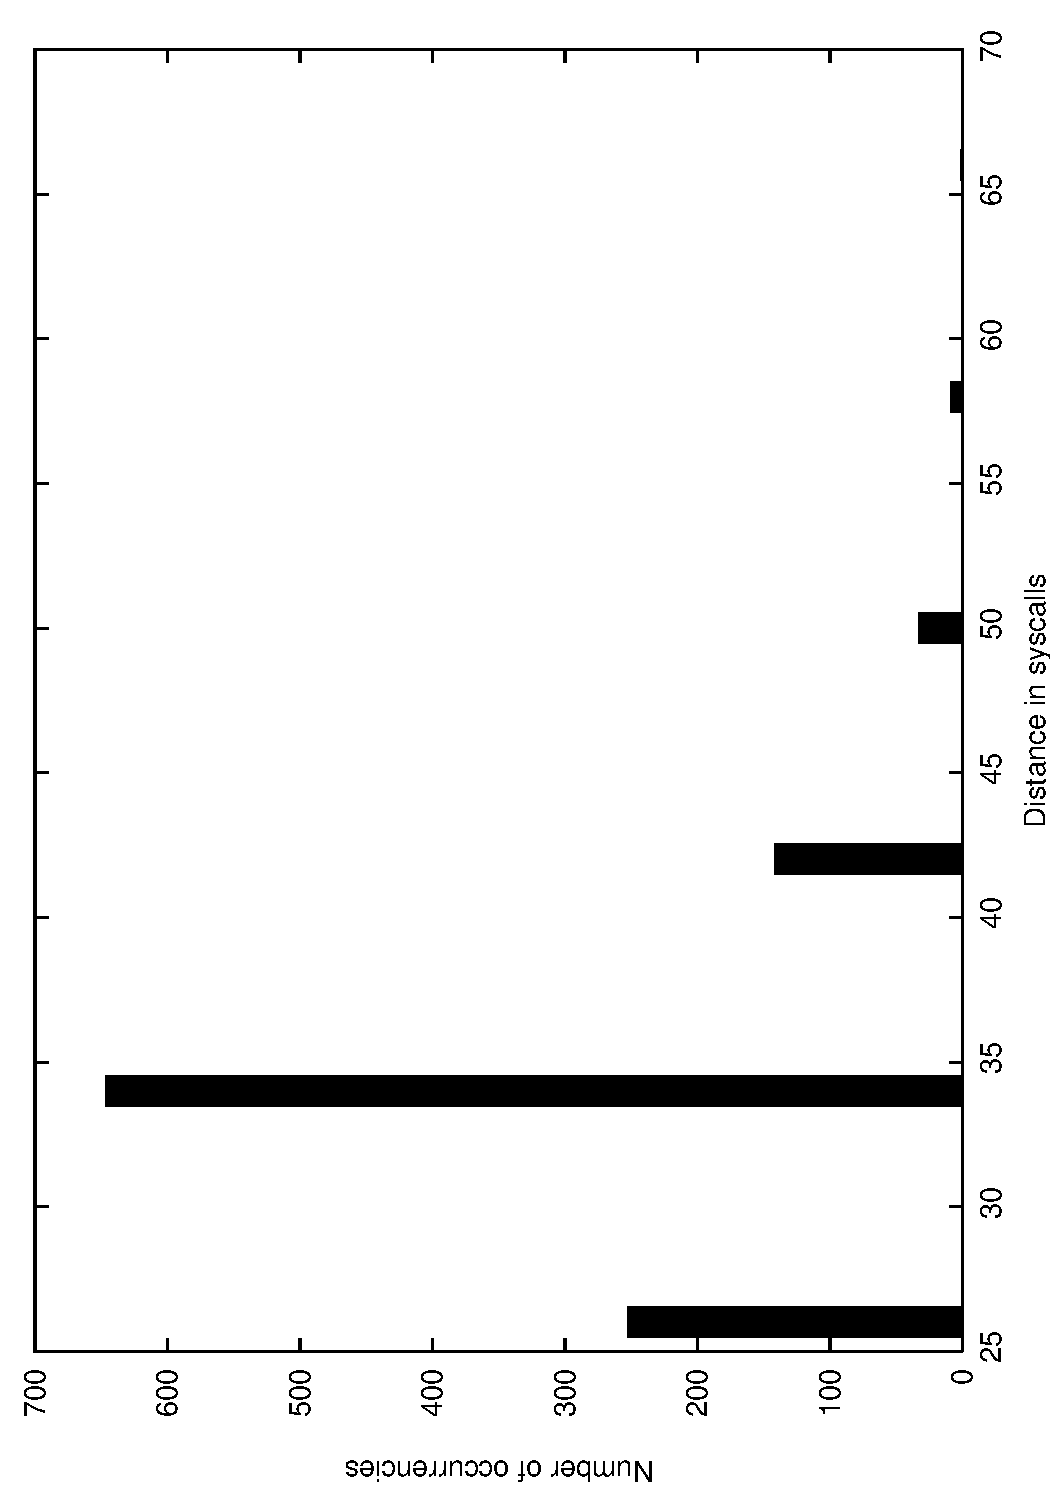
\includegraphics[angle=-90,width=.8\textwidth]{Figures/telnet.pdf}
\caption{\texttt{telnetd}: distribution of the number of other system calls among two \texttt{execve} system calls (i.e., distance between two consecutive \texttt{execve}).}
\label{fig:exectelnet}
\end{figure}

%------------------------------------------------

\section{Bulleted List}

\begin{itemize}
\item $O = $``Intrusion'', $\neg O =$``Non-intrusion'';
\item $A = $``Alert reported'', $\neg A =$``No alert reported''.
\end{itemize}

%------------------------------------------------

\section{Numbered List}

\begin{enumerate}
\item $O = $``Intrusion'', $\neg O =$``Non-intrusion'';
\item $A = $``Alert reported'', $\neg A =$``No alert reported''.
\end{enumerate}

%------------------------------------------------

\section{A Description}

\begin{description}
\item[Time] refers to the use of \emph{timestamp} information, extracted from network packets, to model normal packets. For example, normal packets may be modeled by their minimum and maximum inter-arrival time.
\item[Header] means that the \ac{TCP}\index{TCP} header is decoded and the fields are modeled. For example, normal packets may be modeled by the observed ports range.
\item[Payload] refers to the use of the payload, either at
\ac{IP}\index{IP} or \ac{TCP}\index{TCP} layer. For example, normal packets may be modeled by the most frequent byte in the observed payloads.
\item[Stochastic] means that stochastic techniques are exploited to create models. For example, the model of normal packets may be constructed by estimating the sample mean and variance of certain features (e.g., port number, content length).
\item[Deterministic] means that certain features are modeled following a deterministic approach. For example, normal packets may be only those containing a specified set of values for the \ac{TTL}\index{TTL} field.
\item[Clustering] refers to the use of clustering (and subsequent classification) techniques. For instance, payload byte vectors may be compressed using a \ac{SOM} where class of different packets will stimulate neighbor nodes.
\end{description}

%------------------------------------------------

\section{An Equation}

\begin{equation}
d_a(i,j) := \left\{
\begin{array}{lll}
K_a + \alpha_{a} \delta_{a}(i,j) & \mbox{if the elements are different} \\
0 & \mbox{otherwise}
\end{array}
\right.
\label{eq:distfunction}
\end{equation}

%------------------------------------------------

\section{A Theorem, Proposition \& Proof}

\begin{thm}
$a^2 + b^2 = c^2$
\end{thm}

\begin{prop}
$3 + 3 = 6$
\end{prop}

\begin{proof}
For any finite set $\{p_1,p_2,...,p_n\}$ of primes, consider $m = p_1p_2...p_n+1$. If $m$ is prime it is not in the set since $m > p_i$ for all $i$. If $m$ is not prime it has a prime divisor $p$. If $p$ is one of the $p_i$ then $p$ is a divisor of $p_1p_2...p_n$ and hence is a divisor of $(m - p_1p_2...p_n) = 1$, which is impossible; so $p$ is not in the set. Hence a finite set $\{p_1,p_2,...,p_n\}$ cannot be the collection of all primes.
\end{proof}

%------------------------------------------------

\section{Definition}

\begin{definition}[Anomaly-based \ac{IDS}]
An \emph{anomaly-based \ac{IDS}} is a type of \ac{IDS} that generate alerts $\mathbb{A}$ by relying on normal activity profiles.
\end{definition}

%------------------------------------------------

\section{A Remark}

\begin{rem}
Although the network stack implementation may vary from system to system (e.g., \textsf{Windows} and \textsf{Cisco} platforms have different implementation of \ac{TCP}).
\end{rem}

%------------------------------------------------

\section{An Example}

\begin{example}[Misuse \emph{vs.} Anomaly]\label{ex:misuse-vs-anomaly}
A misuse-based system $M$ and an anomaly-based system $A$ process the same log containing a full dump of the system calls invoked by the kernel of an audited machine. Log entries are in the form:

\begin{center}\small
\begin{verbatim} <function_name>(<arg1_value>, <arg2_value>, ...)
\end{verbatim}
\end{center}
\end{example}

%------------------------------------------------

\section{Note}

\begin{note}[Inspection layer]\label{note:network-stack-standardized}
Although the network stack implementation may vary from system to system (e.g., \textsf{Windows} and \textsf{Cisco} platforms have different implementation of \ac{TCP}), it is important to underline that the notion of IP, TCP, HTTP \emph{packet} is well defined in a system-agnostic way, while the notion of \emph{operating system activity} is rather vague and by no means standardized.
\end{note}
 % Include the first content chapter
%\clearpage

\setcounter{chapter}{2}
\setcounter{section}{0}

% Add the chapter to table of contents
\addcontentsline{toc}{chapter}{\numberline{2}Rethinking Democratization: Beyond Access to Preservation}

\pagestyle{fancy}
\fancyhf{} % Clear all header and footer fields
\fancyhead[L]{\footnotesize\textit{Ars Post Faber: Digital Fabrication Democratization Through Embodied Knowledge Preservation}}
\fancyfoot[C]{\thepage} % Page number in footer center
\renewcommand{\headrulewidth}{0pt}
\renewcommand{\footrulewidth}{0pt}

\noindent
{\Large\textbf{Chapter 2: Rethinking Democratization: Beyond Access to Preservation}}
\vspace{0.3cm}
\hrule
\vspace{0.8cm}
\label{ch:democratization}

% Set no paragraph indentation
\setlength{\parindent}{0pt}

The historical trajectory examined in Chapter 1 has showed how creative agency has been systematically redistributed from unified practice to contemporary digital workflows. This analysis raises the question: if digital fabrication technologies possess unprecedented capabilities for material manipulation and geometric exploration, why do they continue to perpetuate the same distributed agency frameworks that eliminated adaptive authority? The answer lies in how the "democratization" itself has been conceptualized within digital fabrication discourse.

\vspace{0.5cm}

Rather than addressing the organizational structures that fragment creative agency, contemporary digital fabrication has pursued democratization primarily through expanded access to scaled-down industrial tools. This chapter will examine how this access-centered approach, while achieving remarkable quantitative success, fails to address the deeper structural issues identified in the historical analysis. By tracing the evolution from access-based democratization toward preservation-centered approaches, this chapter will try to pursue a reconceptualization of what democratic making might mean in digital contexts.

\section{The Access Paradigm and Its Achievements}

This access-centered understanding of democratization has become the dominant paradigm within contemporary digital fabrication discourse. Neil Gershenfeld's\footnote{Neil Gershenfeld is a physicist at MIT who's the director of the Center for Bits and Atoms (CBA) and pioneered the global FabLab movement. His work focuses on the intersection of physical and digital systems, advocating for "personal fabrication" as a means to democratize access to manufacturing capabilities.} foundational vision for FabLabs\footnote{FabLabs (Fabrication Laboratories) are digital fabrication workshops that provide public access to tools for invention, prototyping and local production. Originally conceived at MIT's Center for Bits and Atoms, FabLabs follow a global charter emphasizing open access, education, and local innovation while connecting to a worldwide network of collaborative spaces.} promised "personal fabrication" enabling "almost anyone to make almost anything" \citep{gershenfeld2007}, positioning digital fabrication as the natural evolution of personal computing—bringing the same accessibility that desktop computers brought to information processing into the realm of physical manufacturing. This vision emphasized scaling down industrial production capabilities to individual users, making sophisticated fabrication tools available in community workshops and educational institutions.

\vspace{0.5cm}

\begin{figure}[h]
\centering
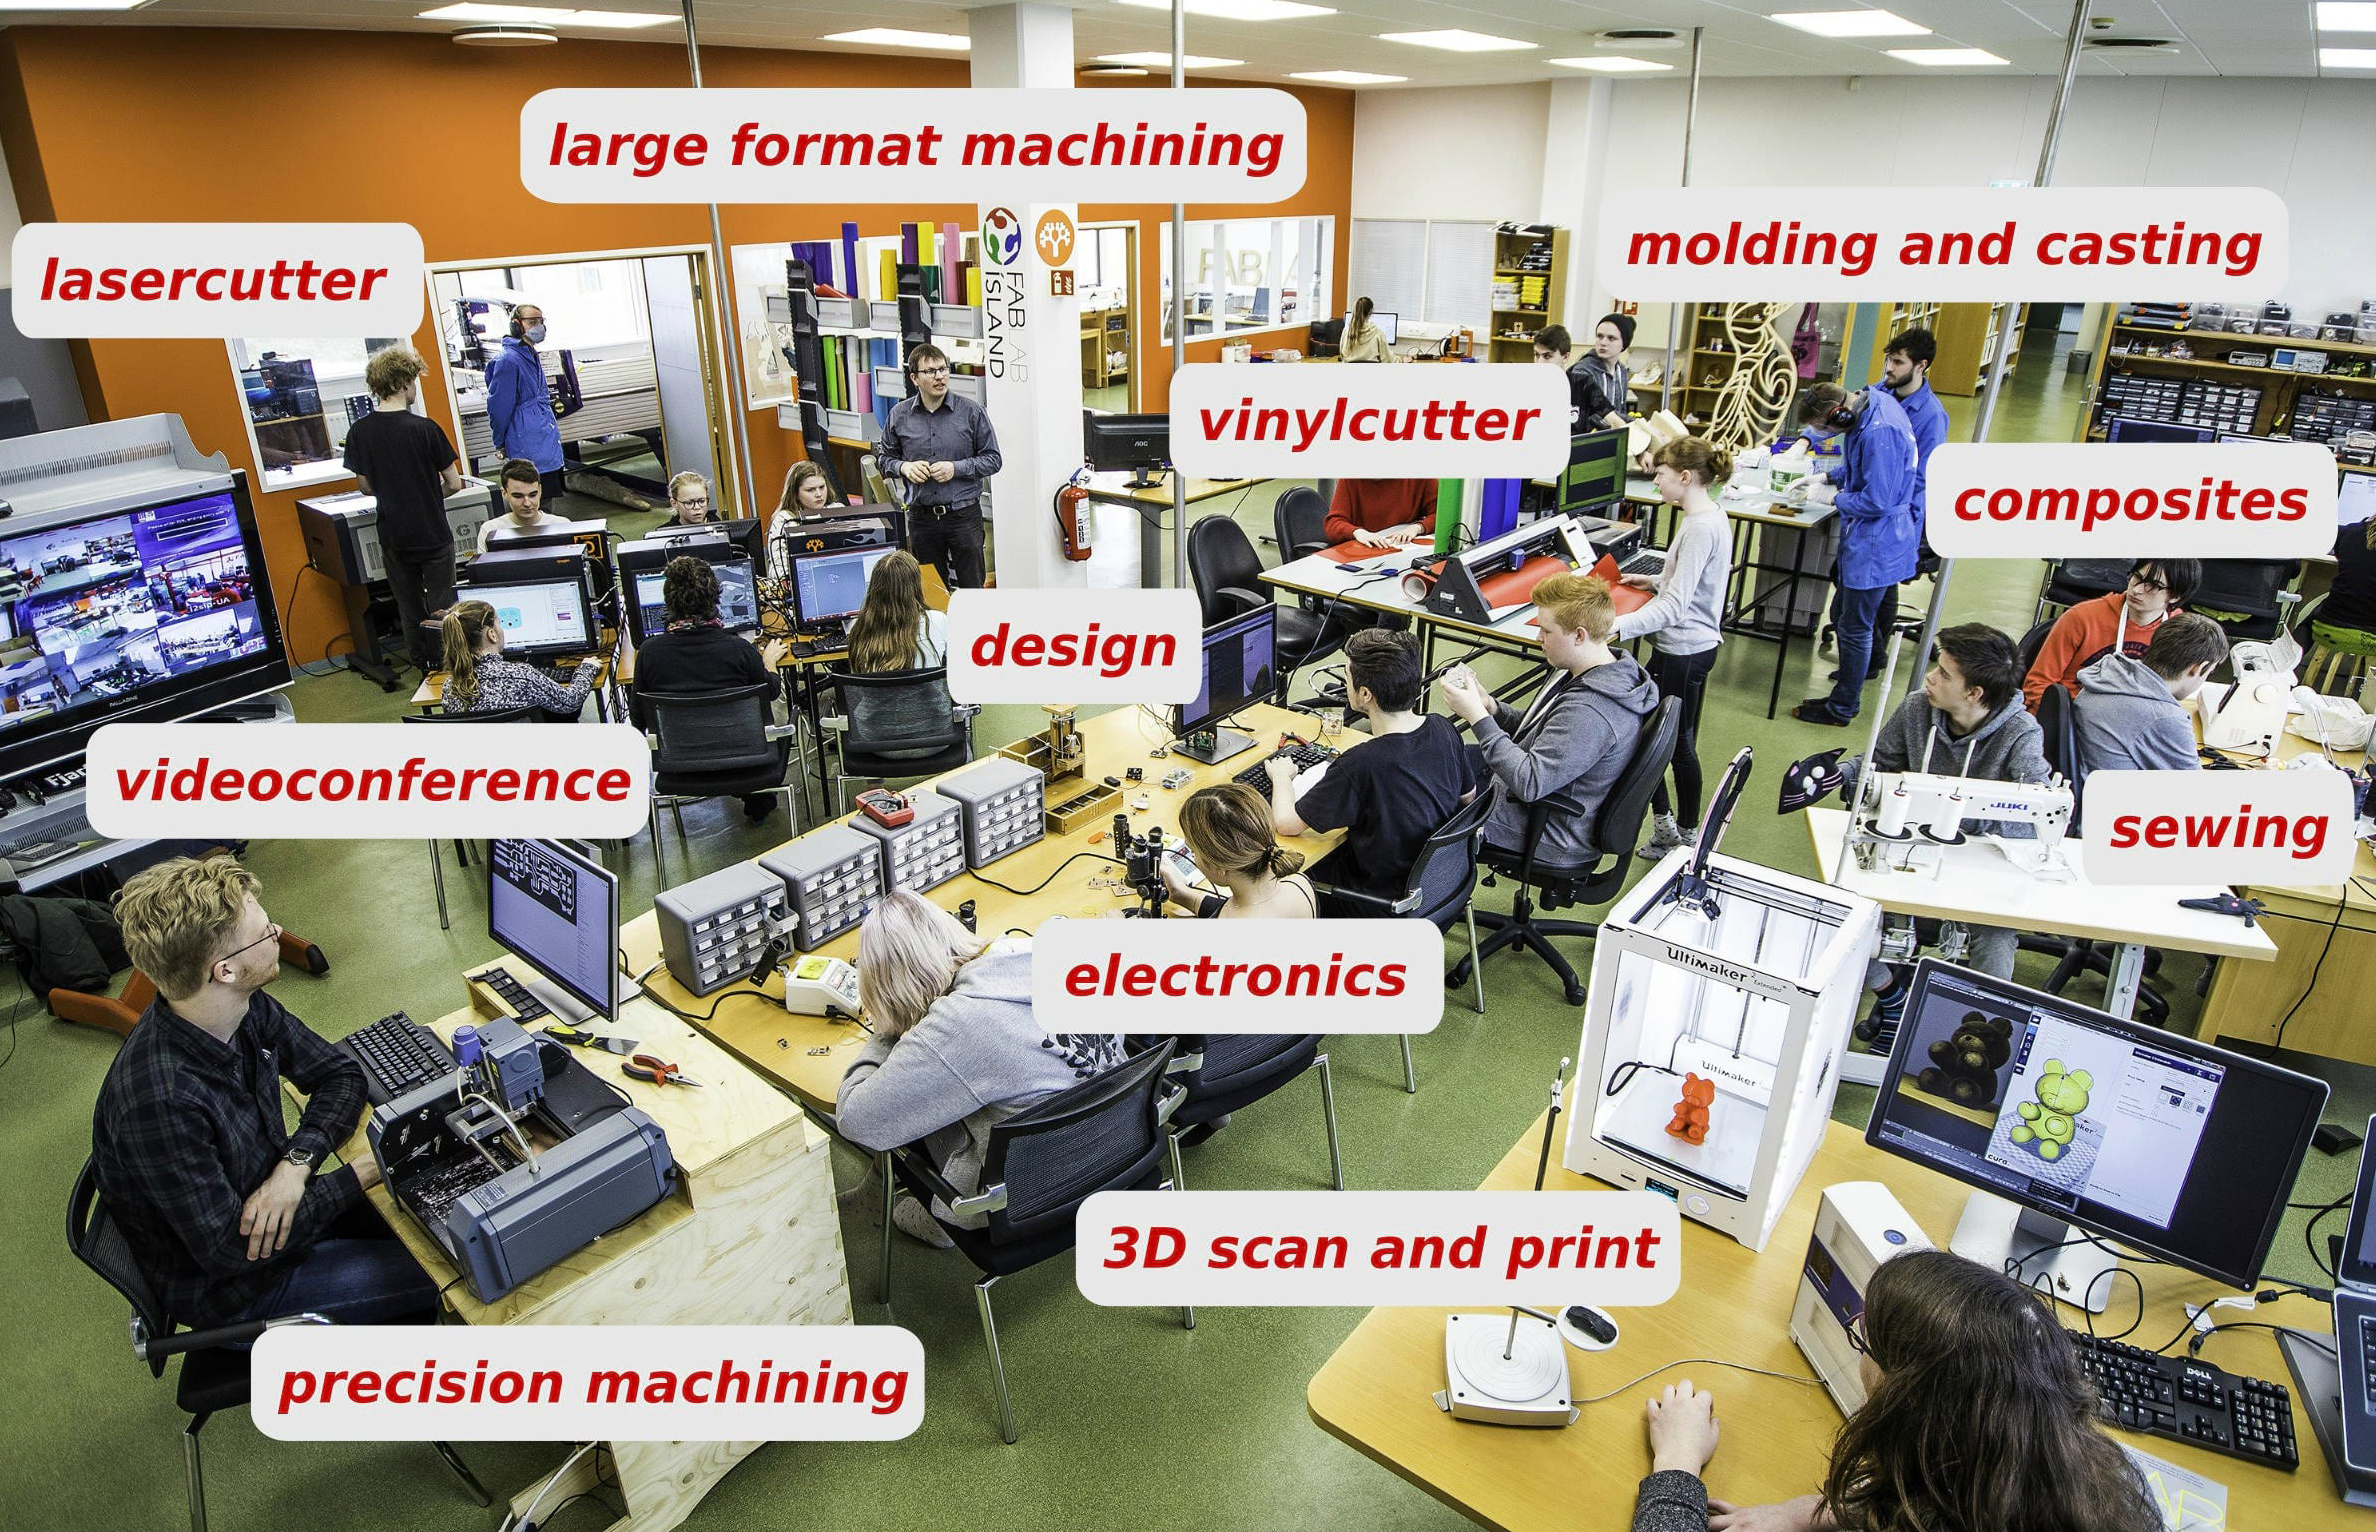
\includegraphics[width=1\textwidth]{figures/chapter2/fablab_tools.jpg}
\caption{Tools in a Fab Lab. Source: Fab Foundation, 2024}
\label{fig:fablab_tools}
\end{figure}

Building on this foundation, the broader maker movement, as articulated by Mark Hatch, advocated for "radically democratizing access to the tools of innovation" \citep{hatch2013}, framing making as both a form of personal empowerment and economic opportunity. Hatch's manifesto positioned the maker movement as a response to mass production's alienation, promising that widespread access to fabrication tools would restore individual agency in production while fostering innovation and entrepreneurship at the grassroots level.

\vspace{0.5cm}

This approach has achieved remarkable quantitative success: from fewer than 50 FabLabs worldwide in 2009 to over 2,000 by 2023 \citep{fabfoundation2024}, there's been an unprecedented expansion of access to sophisticated production capabilities.

\vspace{0.5cm}


\begin{figure}[h]
\centering
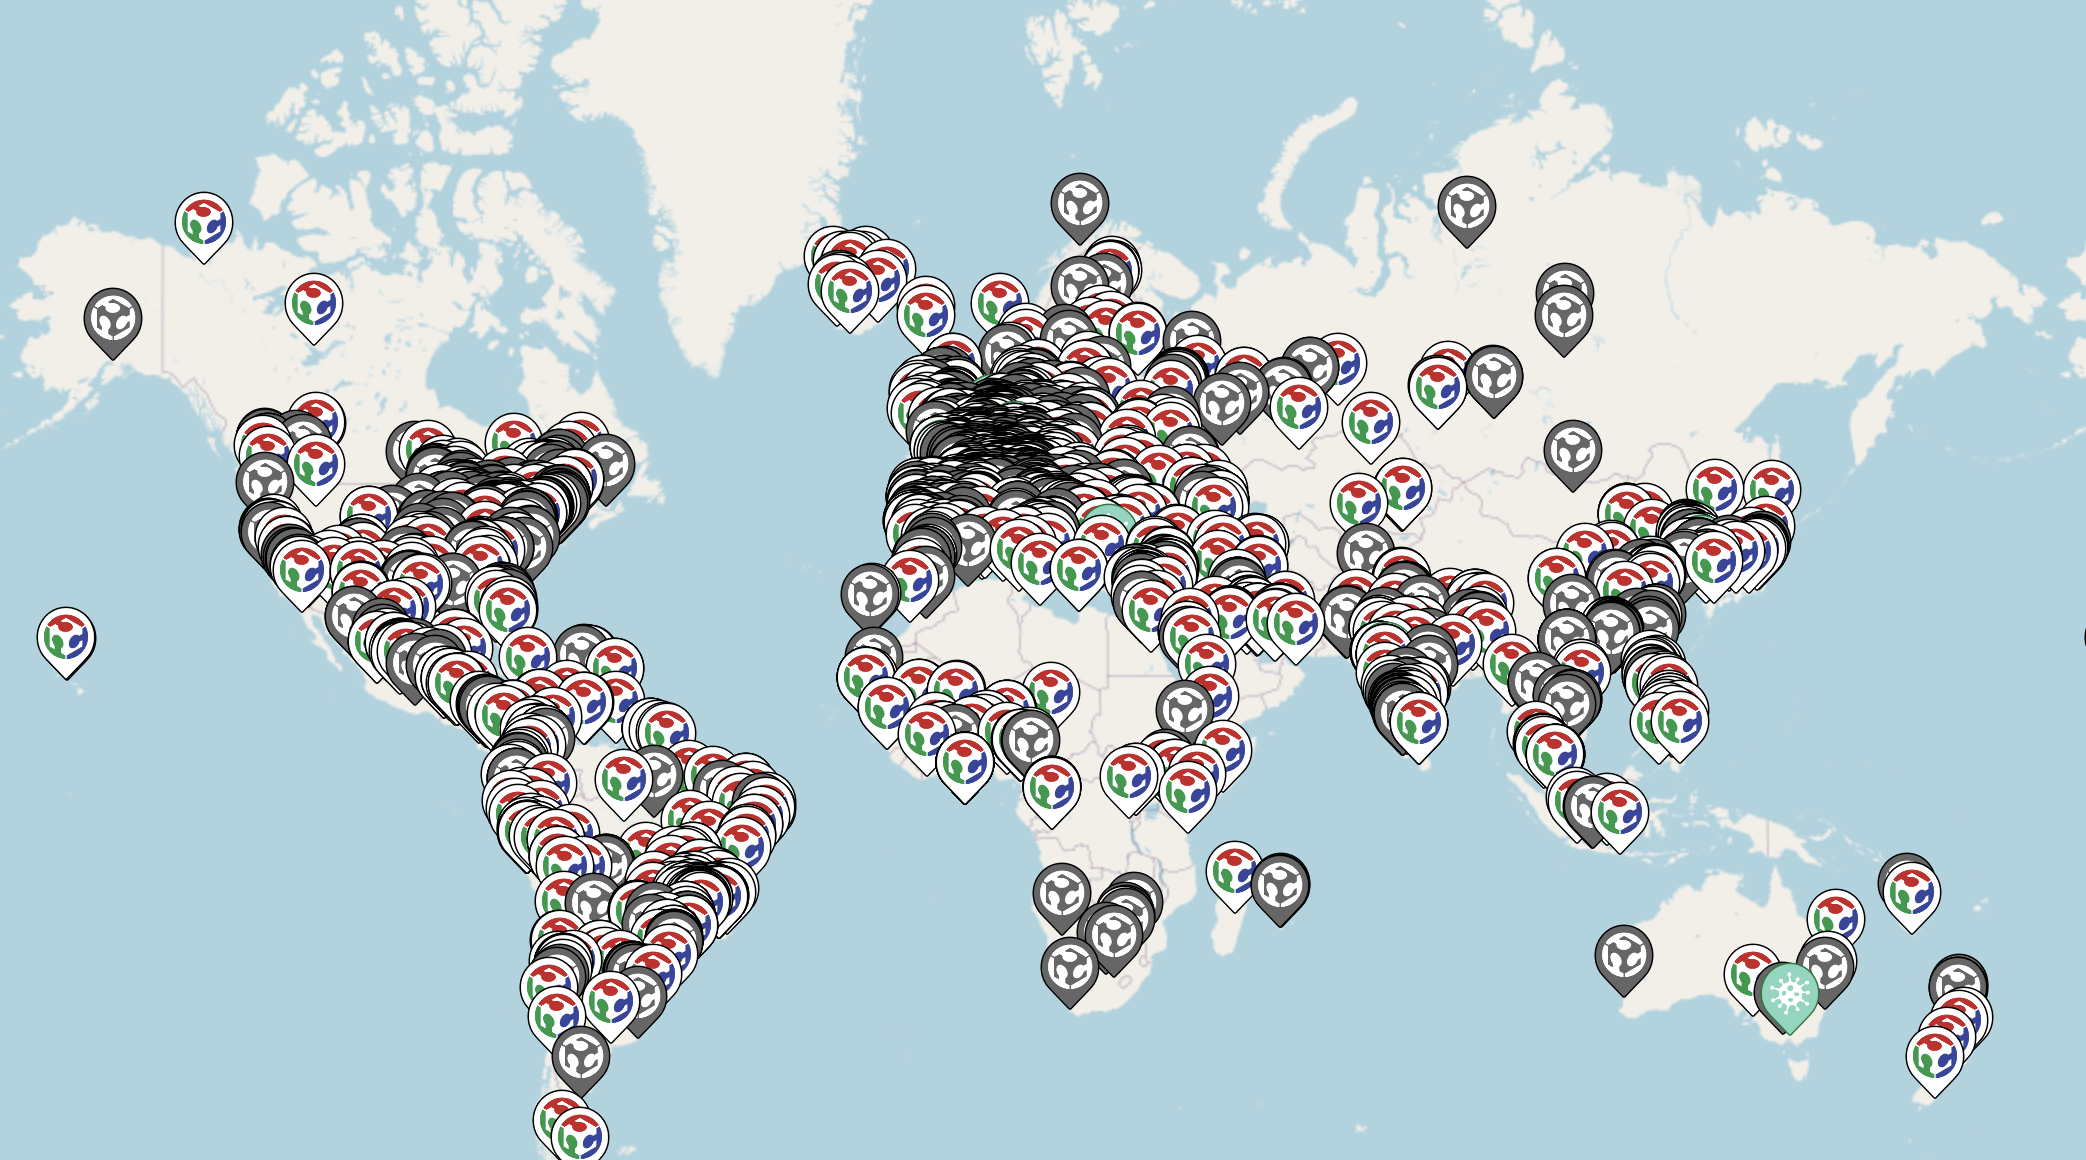
\includegraphics[width=1\textwidth]{figures/chapter2/fablabsmap.png}
\caption{Global distribution of FabLabs. Map showing the locations of FabLabs around the world. Source: Fab Foundation, 2024}
\label{fig:fablabs_map}
\end{figure}

This democratization of digital fabrication extends beyond physical tools to software infrastructures. Open-source\footnote{Open-source software is developed with publicly accessible source code, allowing users to modify, improve the software and in some cases even distribute it.} and free CAD alternatives like FreeCAD\footnote{FreeCAD is a parametric 3D CAD modeler designed for mechanical engineering and product design, available as free and open-source software.}, Blender\footnote{Blender is an Open-Source 3D creation suite supporting modeling, animation, rendering, and video editing, mainly used for animation but increasingly used for CAD applications.} or TinkerCAD\footnote{TinkerCAD is a web-based 3D design application developed by Autodesk, designed for beginners with simplified modeling tools and browser-based accessibility.} combined with educational programs to know how to use the tools, have reduced barriers to digital design literacy. Contemporary maker spaces enable individual access to CNC machines\footnote{Computer Numerical Control (CNC) machines use computer-controlled cutting tools to precisely shape materials like wood, metal, and plastic from digital designs.}, 3D printers\footnote{3D printers create physical objects by depositing material layer by layer based on digital 3D models, enabling rapid prototyping and small-scale production.}, and laser cutters\footnote{Laser cutters use focused laser beams to cut or engrave materials with high precision, commonly used for creating flat parts from sheet materials like wood, acrylic, and metal.} for modest fees (sometimes even for free), genuinely transforming the economic conditions of making.

\vspace{0.5cm}

Yet this access-focused paradigm highlights certain limitations when examined against historical precedents of successful democratization movements. The expansion of who can use fabrication tools does not address how those tools structure agency within making processes. As Tanenbaum et al. observe, maker practices still depend heavily on existing industrial infrastructure and face challenges "when it comes to scaling up production and distribution" \citep{tanenbaum2013}.

\section{The Preservation Problem: What Access Cannot Address}

While the quantitative expansion of fabrication access represents genuine progress, it reveals limitations in how democratization has been conceptualized. What contemporary digital fabrication lacks is what this research identifies as a preservation problem: the loss of tacit knowledge and embodied practices that characterize skilled making. This goes beyond the historical fragmentation patterns analyzed in Chapter 1 to encompass how knowledge itself is transmitted, maintained, and evolved within making communities.

\vspace{0.5cm}

Richard Sennett's analysis of craftsmanship emphasizes that "the desire to do something well for its own sake" \citep{sennet2009} requires forms of embodied learning that resist systematic codification. Unlike explicit knowledge that can be documented in manuals or encoded in software, tacit knowledge emerges through sustained engagement with materials, tools, and techniques.

\vspace{0.5cm}

Contemporary digital fabrication workflows eliminate opportunities for this knowledge transmission. While FabLabs and maker spaces provide access to sophisticated tools, they typically operate through standardized tutorials and predetermined project sequences that prioritize rapid skill acquisition over deep material understanding. The emphasis on "democratizing" access often translates into simplifying workflows to reduce learning curves, eliminating the complex, time-intensive processes through which tacit knowledge traditionally develops.

\vspace{0.5cm}

This preservation problem manifests through persistent organizational structures that extend beyond individual tool use. Despite the collaborative and educational dimensions of maker spaces, the workflow architecture maintains the distributed agency pattern traced in Chapter 1. Creative decisions remain concentrated in separate design phases, while material execution follows predetermined procedures that eliminate opportunities for the responsive adaptation. The result is a democratization that provides access to tools without preserving the knowledge systems that enable those tools to support genuine creative agency.

\vspace{0.5cm}

The insight that emerges from this analysis is that democratization cannot be achieved through access alone, it requires organizational innovation that preserves the continuity of creative decision-making throughout the making process. This shifts focus from who can use fabrication tools to how those tools can be structured to maintain what was identified in Chapter 1 as unified agency. 

\section{Redefining Democratization: Process Over Access}

Through the analysis of the preservation problem it's possible to raise the question about how "democratization" has been conceptualized within digital fabrication discourse. While the term implies expanding democratic participation, current approaches, as mentioned, focus primarily on access expansion rather than examining what democratic participation actually requires. Before proposing alternative models for fabrication democratization, it becomes necessary to question what "democracy" itself demands and how those requirements might apply to making contexts.

\vspace{0.5cm}

The analysis of different precedents and patterns suggest that democratization movements across multiple domains initially focus on access expansion before recognizing deeper structural challenges. Political democratization, educational reform, and cultural preservation movements all showcase patterns that would align with it: early phases emphasize expanding participation within existing systems, while later phases require fundamental transformation of the systems themselves. For instance, political democratization initially focused on expanding voting rights, but later required systematic changes like proportional representation systems such as the D'Hondt method\footnote{The D'Hondt method is a proportional representation electoral system that allocates seats based on vote share, developed to ensure more democratic representation beyond simple majority voting.} to ensure genuine democratic representation rather than mere voting access. Similarly, educational democratization moved beyond simply expanding school enrollment to developing pedagogical approaches that understand and accommodate diversity in the classroom, adapting curricula to different learning styles and cultural backgrounds rather than imposing standardized approaches. These precedents suggest that fabrication democratization may be encountering similar limitations inherent to access-based approaches.

\vspace{0.5cm} 

Rather than assuming that broader tool access automatically produces democratic participation, the following analysis will examine what democracy actually requires and how those requirements might inform alternative approaches to fabrication democratization. By analyzing democratic theory alongside cross-cultural preservation practices, this chapter will attempt to develop frameworks for distinguishing between superficial access and substantive democratic participation in production processes.

\subsection{Deconstructing "Democratization": What Democracy Actually Requires}

The theoretical framework established requires a deeper examination of the term "democratization" itself and its specific application to fabrication contexts. While democratic theory provides extensive analysis of political participation, its principles have been applied to fabrication with insufficient critical examination of what democratic participation might actually require within making processes. The word "democracy" derives from the Greek {\greekfont δημοκρατία} (demokratia) demos (people) + kratos (power/rule), meaning rule by the people. This etymology suggests that democratization involves the distribution of ruling authority rather than expanded access to predetermined systems, a distinction with big implications for how fabrication democratization should be conceptualized.

\vspace{0.5cm}

Political democracy, at its core, requires the distribution of decision-making authority among participants rather than merely access to predetermined decision-making processes. As Robert Dahl's\footnote{Robert A. Dahl (1915--2014) was an American political theorist whose work on democratic theory, shaped contemporary understanding of democratic systems and citizen engagement.} foundational analysis demonstrates, democratic systems must provide "effective participation" \citep{coglianese1990} where citizens have "basic political rights and liberties, such as free expression, and allows persons to live under laws of their own choosing" \citep{coglianese1990}, and enlightened understanding enabling informed choice among alternatives. Crucially, democracy requires what Dahl terms "final control over the agenda" \citep{mayhew2017}, the authority to determine not just outcomes within predetermined options, but the capacity to define what questions get asked and how they are framed. Distinguishing genuine democratic participation from consultative processes that solicit input within predetermined parameters while concentrating agenda-setting authority elsewhere.

\vspace{0.5cm}

Applied to fabrication contexts, this analysis reveals that current maker spaces, despite their collaborative ethos, preserve a fabrication autocracy, a system that concentrates creative authority in separate design phases while relegating material execution to predetermined procedures that eliminate participant agency. Genuine fabrication democratization would require the distribution of creative decision-making authority throughout making processes, enabling makers to exercise "final control over the agenda" not just in initial design specification, but in determining how fabrication workflows themselves operate and evolve in response to material conditions and emergent discoveries.

\subsection{The Representation Problem in Fabrication Democracy}

Having established that genuine democratization requires the distribution of decision-making authority rather than mere access expansion, it becomes necessary to examine how such authority might be structured within fabrication contexts. Political democracy usually confronts the challenge of representation: how to enable large-scale collective decision-making while preserving individual agency? This requires sophisticated institutional frameworks, electoral systems, deliberative processes, and constitutional protections that mediate between individual preferences and collective outcomes without eliminating personal autonomy.

\vspace{0.5cm}

Fabrication democratization faces analogous representational challenges: how to enable collective access to sophisticated manufacturing capabilities while preserving individual makers' authority to determine their own creative processes? Yet current digital fabrication has developed no equivalent to democratic political institutions. Instead, it has adopted  a technocratic representation, expert-designed software interfaces and standardized file formats that mediate between human intention and material execution while eliminating opportunities for maker input beyond initial design specification.

\vspace{0.5cm}

This technocratic approach mirrors Joseph Schumpeter's\footnote{Joseph Schumpeter (1883-1950) was an Austrian economist and politic who developed influential theories about capitalism and democratic systems.} theory of democracy as "competitive leadership" \citep{schumpeter1950}, a system that preserves formal democratic procedures while concentrating substantive decision-making authority within expert institutions. Just as this limited democracy enables citizen participation within predetermined choices while eliminating popular control over the agenda setting, just as current fabrication democratization enables maker participation within predetermined expert designed workflow structures while eliminating authority over how those structures have to be operated.

\subsection{Participatory Democracy and Making}

The technocratic representation reflects what participatory democratic theorists have long criticized in conventional political systems. Rather than accepting the limited model of democracy as competitive leadership, theorists like Carole Pateman advocate for democracy as active participation across all spheres of social life, "a society where all political systems have been democratised and socialisation through participation can take place in all areas" \citep{pateman1976}. Pateman argues that democratic capacity cannot be developed through formal instruction alone but emerges through the practice of exercising democratic authority in concrete contexts.

\vspace{0.5cm}

For fabrication democratization, out of this participatory approach can be extracted that creative agency develops itself through sustained engagement with decision-making throughout the making process rather than through standardized training in predetermined procedures. This would challenge the separation between tool designers and tool users that characterizes current maker spaces, and processes, requiring structures that enable makers to collectively determine how fabrication workflows themselves operate and evolve. Instead of accepting expert-designed workflow structures as fixed constraints, participatory fabrication would enable makers to exercise that "final control over the agenda".

\section{Deconstructing "Preservation": Beyond Cultural Heritage Models}

Out of the democracy framework outlined in this research can be assumed that genuine fabrication democratization requires preserving makers' capacity for ongoing creative authority rather than simply expanding access to predetermined tools. This shifts the focus from "democratization" as access provision to "democratization" as preservation of agency. But what kind of preservation enables rather than constrains democratic participation? The concept of "preservation" itself requires an examination, as its application to craft knowledge has been heavily influenced by cultural heritage frameworks that reproduce the same static approaches that align with access-based democratization.

\vspace{0.5cm}

Understanding preservation through cross-cultural perspectives can reveal assumptions embedded within Western conservation models and might highlight alternative approaches more suitable for maintaining the creative agency that democratic fabrication requires.

\subsection{Preservation as Dynamic Process vs. Static Conservation}

Traditional cultural preservation models, developed primarily for archaeological, crafts, and architectural contexts, emphasize conservation of existing artifacts and documentation of historical practices. This approach, rooted in western "museum culture", treats cultural objects as fixed entities requiring protection from change rather than as elements within ongoing living traditions that respond to new conditions and challenges.

\vspace{0.5cm}

The 2003 UNESCO Convention for the Safeguarding of Intangible Cultural Heritage marked a shift in this perspective by recognizing that cultural heritage extends beyond tangible things to include "identification, documentation, research, preservation, protection, promotion, enhancement, transmission" \citep{unesco2003}. More importantly, the convention defines intangible cultural heritage as something that is "constantly recreated by communities and groups in response to their environment" \citep{unesco2003}, explicitly acknowledging its living, evolving nature.

\vspace{0.5cm}

However, this framework still emphasizes documenting and officially recognizing traditional practices rather than preserving communities' ability to adapt and change those practices. The UNESCO approach, while acknowledging living practices, still requires processes that tend to crystallize traditions into documentable forms rather than preserving their adaptive capacity, the quality that democratic fabrication systems must maintain to enable ongoing maker authority over creative processes.

\subsection{Cross-Cultural Models of Adaptive Preservation}

The static documentation approaches critiqued highly contrast with preservation practices across different cultural contexts that prioritize maintaining agency and adaptive capacity over material authenticity. These alternative models demonstrate how preservation can support the kind of ongoing democratic authority that participatory fabrication requires.

\subsubsection{Cuban Automobile Preservation: Functionality Through Adaptation}

Cuba's preservation of classic American automobiles exemplifies a functional preservation, the maintainance of cultural significance through continuous adaptation oposed to static conservation. Following the 1959 Cuban Revolution and subsequent U.S. embargo, Cubans maintained an estimated 60,000 classic American cars through creative adaptation. As the \citet{diplomatictimes2019} reports, "About half of the cars originate from the 1950s, while 25 percent are from the 1940s and another 25 percent are from the 1930s. A lot of them have been passed down from generation to generation, along with the mechanical genius."

\vspace{0.5cm}

These vehicles remain culturally significant not despite their modifications but because of them. Their external appearancespreserve historical recognition value while their internal systems have evolved into hybrid assemblages. "A common substitution on the old 1950s era cars on the island are diesel engines for the old straight-six or V-8 engines originally in the cars, due to diesel's lower cost on the island, and the better fuel efficiency of the engines," \citep{diplomatictimes2019} with "diesel engines from Russian trucks or boats" \citep{diplomatictimes2019} replacing original components.

\vspace{0.5cm}

This preservation approach prioritizesthe ongoing functionality and cultural continuity over "strict" tangible authenticity. The cars remain integrated within contemporary Cuban life, functioning as taxis and tourist attractions rather than museum pieces, showcasing preservation through active use rather than protection from use. As \citet{adewale2024} observes, "While some people might expect these old cars to be museum pieces, they're part of everyday life in Cuba."

\subsubsection{Māori River Preservation: Relational Continuity Through Legal Innovation}

New Zealand's legal recognition of the Whanganui River as a living entity with "the same rights and responsibilities as a person" \citep{paremata2017} exemplifies preservation through transformed conceptual frameworks rather than material conservation. This approach emerged from Māori understanding expressed in the saying "Ko au te awa, ko te awa ko au" (I am the river, and the river is me), where the river name "Awa Tupua" includes "the whole river system, its spirit, and the people that are related to it" \citep{nationallibrarynz2017}.

\vspace{0.5cm}

Rather than treating the river as a natural resource requiring protection through regulatory restriction, this model empowers the Māori to manage and protect the river based on their traditional ecological knowledge. As \citet{vijaykuma2019} notes, "As a consequence of this recognition, the Maori are now empowered to manage and protect the river based on their traditional ecological knowledge." Preservation here operates through maintaining relationships and ongoing interactions rather than controlling physical attributes or preventing change.

\vspace{0.5cm}

This relational approach recognizes that preservation must account for living connections between people, practices, and environments rather than treating cultural elements as discrete objects requiring isolation from contemporary influences.

\subsubsection{Implications for Digital Fabrication Democratization}

These diverse preservation models highlight shared principles that might address the democratization challenges identified earlier. Both Cuban functional adaptation and Māori relational continuity prioritize process over product, relationships over artifacts, and adaptation over stasis. As \citet{munoz_zanon_2025} concludes from this analysis, effective preservation approaches should "capture process knowledge and decision-making rather than just final geometries, preserve the dynamic relationship between maker, material, and tool, and allow for adaptation and evolution rather than freezing techniques in time."

\vspace{0.5cm}

Taking a look at the fabrication democratization aspect, out of these principles it can be asummed that preserving makers' agency requires organizational structures that maintain what the Cuban model showcases: the capacity for ongoing functional adaptation in response to changing conditions. Similarly to the Māori approach, genuine fabrication democratization would preserve makers' collective authority to determine how systems evolve, maintaining the relational continuity between human intention and material response.

\section{Documentation as Process Preservation}

The preservation approaches demonstrated by Cuban mechanics and Māori river stewardship raise questions about how digital fabrication systems might maintain makers' adaptive authority. These become particularly present when examining how fabrication knowledge is documented and transmitted. Current fabrication documentation perpetuates the technocratic representation characteristic of the distributed agency model, enabling participation within predetermined procedures while eliminating authority over how those procedures operate. Standard fabrication documentation (CAD files, parameter lists, step by step tutorials\dots) work as expert-designed interfaces that mediate between human intention and execution, eliminating opportunities for creative input beyond initial design specification.

\vspace{0.5cm}

However, examining documentation practices across different contexts reveal alternative approaches that align better with the dynamic preservation principles and participatory democratic theory already examined.

\subsection{Educational Documentation: Capturing Learning Processes}

The FabAcademy\footnote{FabAcademy is a global distributed educational program that teaches digital fabrication skills through hands-on learning and peer-to-peer collaboration. Students work through weekly assignments using local Fab Lab equipment while documenting their progress online.} and Fabricademy\footnote{Fabricademy is a transdisciplinary course that focuses on the development of new technologies and materials for the textile and fashion industry, emphasizing bio-fabrication, digital manufacturing, and sustainable design practices.} documentation sites provide examples of documentation that capture learning processes besides just technical outcomes. Unlike traditional technical manuals that present polished procedures, these educational platforms require students to document their entire learning journey, including failed experiments, debugging processes, and iterative refinements. Students document not only successful fabrication outcomes but also the problem-solving processes that led to those outcomes, creating records of adaptive authority.

\vspace{0.5cm}

Fabricademy specifically, becomes an interesting example as it extends this approach to textile and bio-material fabrication, where material unpredictability requires even greater adaptive capacity. Students document experiments with living materials and organic processes where following predetermined procedures often fails, and creative adaptation becomes essential. The resulting documentation captures the iterative process of material negotiation that can also be seen in traditional craft knowledge.

\subsection{Workflows as Narrative Preservation}

Tandem system \citep{tran_oleary_tandem_2024} represents another interesting approach to process-oriented documentation, implementing entire fabrication workflows as computational notebooks that preserve the complete narrative of creation. Rather than abstracting away the making process into separate CAD/CAM phases, Tandem maintains continuity between design decisions and material execution through "reproducible fabrication workflows" \citep{tran_oleary_tandem_2024}.

\vspace{0.5cm}

Interestingly, the project acknowledges that reproduction is not repetition, each implementation involves contextual adaptations based on available materials, equipment variations, and maker expertise. By implementing workflows as modifiable programs rather than fixed procedures, the system enables a generative reproduction, allowing to maintain creative agency while building on previous work, representing a significant switch from standard CAD/CAM workflows that concentrate creative decisions in separate design phases.

\section{The Limits of Algorithmic Preservation}

While these educational documentation approaches highlight promising alternatives to static preservation, they still operate within digital systems that fundamentally assume craft knowledge can be captured and transmitted through explicit documentation. This assumption has led contemporary approaches toward an even more technologically intensive solution: artificial intelligence and machine learning as comprehensive approaches to preserving and transmitting embodied knowledge. Suggesting that if human documentation proves inadequate, computational systems might decode the embodied knowledge through pattern recognition and data analysis.
\vspace{0.5cm}

However, machine learning approaches to kowledge preservation create a paradox: the more precisely algorithms attempt to measure and classify skilled practice, the more they help discover dimensions of that practice that resist an algorithmic categorization. This suggests that the problem with embodied knowledge preservation may not be inadequate computational architectures, but rather the conceptual framework that treats embodied knowledge as extractable data rather than contextual relationships between makers, materials, and tools.

\subsection{Testing the Limits of preservation. AI.RTISANSHIP}

Even with the aforementioned problems with algorithmic approaches to craft preservation, these "limitations" demanded empirical investigation. If computational systems truly cannot capture the adaptive authority that democratic making requires, this assumption needed testing through direct experimentation. To investigate these limitations empirically, this research developed as a first intervention the AI.RTISANSHIP experiment, an attempt to capture and digitize traditional pottery techniques through computer vision and machine learning systems, designed not to succeed but to reveal precisely where and why such approaches fail.

\vspace{0.5cm}

The goal was to create a machine learning model capable of analyzing artisanal hand movements and providing real-time feedback on the correctness of performed actions, essentially functioning as a "digital master" for craft learning. By pushing algorithmic preservation to its technical limits, the experiment aimed to identify the specific dimensions of craft knowledge that resist computational capture, thereby informing alternative future approaches.

\subsection{Technical Developement: Digitizing Embodied Knowledge}

The AI.RTISANSHIP system made use of MediaPipe's holistic model to track 33 pose landmarks, 21 landmarks per hand, and facial features, generating 225-dimensional vectors for each frame of movement. The machine learning pipeline processed sequences of 30 frames (approximately one second of movement) through a three layer bidirectional LSTM network with dropout regularization and L2 penalty terms to prevent overfitting.

\vspace{0.5cm}

Data collection involved recording multiple pottery throwing sessions, manually labeling frame collections of movements as "correct" or "incorrect," and training the neural network to recognize these patterns in unseen views. The system achieved accuracy in distinguishing between predefined movement categories, successfully identifying differences between throwing techniques and providing real-time classification through a web interface.

\vspace{0.5cm}

However, this technical "success" started highlighting conceptual issues mentioned before that only became apparent through the extended testing with the potters.

\subsection{The "Unmeasurable" Dimensions of Knowledge}

The experiment's concluded that craft knowledge works through dimensions that resist algorithmic capture. Computer vision could detect hand positions with great precision but remained blind to the tactile feedback that made those positions, the subtle resistance of clay indicating proper centering, texture changes indicating moisture, or vibrations warning of collapsation. These sensory channels, essential for pottery practice, exist entirely outside the visual domain that computer vision systems can access.

\vspace{0.5cm}

Beyond these sensory limitations, the experiment exposed deeper problems with the assumption that skilled practice follows standardizable patterns. Each participating artisan showcasded different approaches to identical pottery tasks, reflecting not just technical variations but personal relationships with clay developed through years of individual practice. Where one potter might relied on strong decisive movements, another employed gentle, patient techniques. These differences stemmed not from varying levels of skill but from unique personal histories, physical capabilities, and aesthetic preferences that had developed into distinct making "philosophies".

\vspace{0.5cm}

In it's core, the machine learning system's requirement for binary classification ("correct" versus "incorrect") proved conceptually inappropriate for pottery practice. The participating potters emphasized that successful throwing depends on continuous adaptation to emergent material conditions rather than adherence to predetermined techniques. This adaptive capacity, cannot be reduced to pattern recognition algorithms that require standardized input categories. Where pottery expertise emerges from continuous dialogue between maker and material, the AI system imposed predetermined classifications that eliminated precisely the adaptive responsiveness that characterizes skilled practice.

\subsection{Implications for Digital Fabrication Preservation}

The real-time feedback mechanism (color-coded overlays indicating "correct" or "incorrect" movements) created additional problems that highlighted even further the inadequacy of the approach. The potters, despite acknowledging the potential of the tool for educational purposes, reported that the visual feedback disrupted their attention to tactile cues. The system's focus on visual movement patterns diverted attention from the sensory channels through which pottery expertise actually operates.

\vspace{0.5cm}

The attempt to extract explicit rules from embodied practices assumes that skilled knowledge can be decomposed into discrete, transferable components. Yet the experiment, as was guessed before starting it, demonstrated that pottery expertise exists not in specific movements but in the capacity for contextual adaptation, precisely what the machine learning system eliminated through its standardized classifications.

\vspace{0.5cm}

Out of these findings, it is possible to suggest that effective craft preservation cannot operate through documentation technologies that abstract away material context and environmental variation.

Effective preservation, would need to maintain the conditions for adaptive response rather than understanding standardized procedures. Representing a shift from traditional documentation based approaches towards a preservation method that maintain the organizational structures only, enabeling ongoing creative adaptation.

\subsection{Beyond Documentation: Toward Ecological Preservation}

Experiment's limitations do not suggest fully abandoning documentation altogether, but rather reconceptualizing what documentation means within embodied knowledge preservation contexts. Documentation remains essential, but it must acknowledge that each implementation of documented knowledge will necessarily differ based on contextual variables, material conditions, and individual maker characteristics.

\vspace{0.5cm}

Rather than attempting to capture universal techniques through computational standardization, effective preservation requires documentation frameworks that explicitly account for contextual variation. This involves creating technological environments that preserve not just movement patterns but the decision-making processes that inform adaptive responses to changing conditions. Such systems would document the reasoning behind technical choices, the environmental factors that influence material behavior, and the range of acceptable variations rather than singular "correct" procedures.

\vspace{0.5cm}

This contextual approach to documentation would treat preservation as the maintenance of conditions for ongoing creative adaptation. Digital fabrication systems (or workflows) designed according to these principles would preserve material feedback channels, enabling real-time modification based on emergent conditions, and maintain maker authority. Documentation would function as a scaffold for contextual learning rather than a template for mechanical reproduction.

\vspace{0.5cm}

The following chapters will explore how such contextually-aware preservation might operate within digital fabrication workflows, building on the AI.RTISANSHIP experiment's insights to develop newer approaches for preservation, reflecting the unique intersection of maker, material, and circumstance.































































 % Include the second content chapter
%\clearpage

\setcounter{chapter}{3}
\setcounter{section}{0}
% Add the chapter to table of contents
\addcontentsline{toc}{chapter}{\numberline{3}From Theory to Practice - Experimental Pathways}


% Set up page style for this chapter (assuming fancyhdr is loaded in preamble)
\pagestyle{fancy}
\fancyhf{} % Clear all header and footer fields
\fancyhead[L]{\footnotesize\textit{Ars Post Faber: Digital Fabrication Democratization Through Embodied Knowledge Preservation}}
\fancyfoot[C]{\thepage} % Page number in footer center
\renewcommand{\headrulewidth}{0pt}
\renewcommand{\footrulewidth}{0pt}


% Custom chapter title to match abstract formatting
\noindent
{\Large\textbf{Chapter 3: Developing Theory From Practice, Experimental Pathways}}
\vspace{0.3cm}
\hrule
\vspace{0.8cm}
\label{ch:experimental_pathways}

% Set no paragraph indentation
\setlength{\parindent}{0pt}
The theoretical framework developed in the previous chapters suggested that genuine democratization of digital fabrication requires preservation-based approaches that maintain adaptive authority rather than simply expanding access to predetermined tools. Yet this analysis raised questions about implementation: \textit{How might such preservation actually operate within existing technological contexts?} \textit{Could alternative "interfaces" bridge the gap between computational precision and embodied expression?} The following interventions sought to address these questions through practical experiments that tested the theoretical propositions in real-world making contexts.

\vspace{0.5cm}

This chapter will document different "interventions" that progressively refined approaches to preserving the embodied knowledge within digital workflows. Each experiment built upon insights from the previous, leading to the development of Ars Post Faber, the open-source Grasshopper\footnote{Grasshopper is a visual programming language and environment that runs within the Rhinoceros 3D computer CAD software. Developed by David Rutten at Robert McNeel \& Associates, Grasshopper enables users to build generative algorithms through a node-based interface without requiring traditional programming knowledge, making it widely used in parametric design, digital fabrication, and computational design workflows.} plugin\footnote{A plugin (also called an add-on or extension) is a software component that adds specific functionality to an existing program. In the context of CAD and design software, plugins extend the applications capabilities by providing new tools, commands, or workflows. They are typically developed by third parties and can be installed and removed without modifying the main software, allowing users to customize their design environment for specific tasks or methodologies.} that embodies the research's theoretical conclusions.

\section{\textit{CR3ATED}: Reimagining CAD Interfaces for Artisan Expression}
\textit{"If craftsmanship's essence lies in the creative problem solving process, how can digital fabrication tools become active participants in it rather than automation devices?"}

\vspace{0.5cm}

\subsection{Exploring Alternative Interface Approaches}

Building upon insights from AI.RTISANSHIP, it was concluded that computational systems could successfully capture and analyze certain patterns of skilled movement, yet this technical capability highlighted a bigger challenge where the preserved data represented only "surface" manifestations of embodied knowledge rather than the adaptive reasoning processes. This raised a different question: \textit{Rather than attempting to extract embodied knowledge from practitioners, what if digital tools could be designed to better support and amplify the adaptive decision-making processes that characterize skilled practice?}

\vspace{0.5cm}

This inquiry led to the development of \textit{CR3ATED}, a web-based application designed to test alternative interface approaches within digital design and fabrication workflows. Where AI.RTISANSHIP looked to decode existing craft knowledge through computational analysis, \textit{CR3ATED} explored how interface design itself might preserve creative expression by exploring different human-software interactions.

\vspace{0.5cm}

The \textit{CR3ATED} experiment investigated whether alternative modes of human-software interaction could maintain the continuity between creative intention and material execution that conventional CAD workflows tend to fragment. The central hypothesis was that interface design actively constructs the kinds of creative relationships that become possible within digital fabrication workflows, suggesting that preserving craft agency might require different approaches to how makers engage with computational design tools.

\subsection{Craftinnova: Testing Alternative Interfaces}

The CR3ATED web application was developed specifically for the "Nuevos Métodos de Aprendizaje Artesano" workshop at CRAFTINNOVA\footnote{CRAFTINNOVA is Spain's national event combining artistic crafts and innovation, held annually in Valladolid. The event brings together creators, designers, manufacturers, technology experts, digital fabrication professionals, artists, entrepreneurs, and makers to explore the intersection of traditional craftsmanship with digital technologies.}, creating an opportunity to test these alternative interface approaches with practicing artisans in a real-world context. The workshop brought together traditional craftspeople with clay 3D printing technology, creating an ideal laboratory for investigating how interface design affects the preservation of creative expression.

\vspace{0.5cm}

Rather than using conventional CAD software, the webapp, implemented a touch-based sketching interface that allowed participants to create 3D models through direct manipulation on mobile devices. The application translated 2D sketches into revolution surfaces suitable for clay printing, maintaining the intuitive hand-to-head connection that characterizes crafts while engaging with the digital fabrication capabilities of the machine.

\vspace{0.5cm}

This approach acknowledged that conventional CAD systems fail to express the imperfection and responsiveness from the craft practice. By creating a workflow that began with tactile sketching and culminated with material engagement, the experiment explored how technology might contribute to craft preservation by becoming integrated into evolving creative practice rather than replacing traditional methods.

\subsection{Material Continuity and Digital Mediation}

An important aspect of the workflow developed involved preserving material continuity between digital design and physical fabrication. The clay printer, despite its digital control system, interacts with clay according to the same physical principles that govern hand techniques, unlike the normally used polymers in additive manufacturing that cannot be hand-treated. Clay maintains its material properties regardless of whether it is shaped by hand or extruded through a mechanical nozzle, maintaining material coherence across the digital/physical boundary.

\vspace{0.5cm}

This materiality creates productive constraints rather than arbitrary limitations. Workshop participants encountered the clay printer's capabilities and limitations as a new set of material conditions to navigate, drawing on their traditional knowledge while developing new skills specific to the printer. Unlike conventional CAD/CAM workflows that abstract away material properties through geometric representation, the \textit{CR3ATED} approach maintained material feedback throughout the process.

\vspace{0.5cm}

The touch interface proved to be important for preserving this material relationship. Whereas CAD requires learning abstract geometric manipulation techniques, sketching with the finger or a stylus maintains the tactile connection between hand movement and form development. Participants of the workshop were able to leverage their existing skills while engaging with digital fabrication, rather than having to master entirely new representational systems.

\subsection{Expanding vs. Replacing Practice}

The workshop generated diverse responses from the participants, showing different ways that digital tools might relate to traditional practice. For most, the clay printing process represented a new exploration rather than a shift in their approach. These artisans engaged with the technology as they might with any new tool or technique, integrating it within their existing practice. However, other participants experienced the workshop as an expansion of their literacy in both digital and material domains. For these makers, the interface exploration enabled forms of creative expression and production that would have been difficult (or impossible) to achieve through either traditional hand-building or conventional CAD approaches.

\vspace{0.5cm}

At it's core, the workshop attempted to challenge the binary thinking that has historically characterized discussions of technology and craft. Rather than facing off hand-building versus digital printing as competing methodologies, the comparison between techniques became "an exploration of their complementary strengths" rather than a contest between "superior" and "inferior" approaches. Aligning with Gershenfeld's vision of personal fabrication enabling the convergence of industrial production with personal expression, "which would merge with digital design, to bring common sense and sensibility to the creation and application of advanced technologies" (Gershenfeld, 2007). The clay printer became not merely a tool but a participant in creative dialogue, presenting its own challenges and possibilities while requiring new skills that built upon traditional knowledge.

\vspace{0.5cm}

\subsection{Success and Limitations of the Experiment}

Despite the "success" in exploring a new way of interaction and preserving material relationships, the intervention highlighted certain limitations that pointed towards the need for more sophisticated future experiments. While the touch-based sketching approach built upon CAD's geometric interaction constraints, it remained limited to revolution forms suitable for lathe operations. Participants could only create objects that could be generated by rotating a 2D profile around an axis.

\vspace{0.5cm}

More importantly, the simplification required to make this interface accessible to users with no CAD experience eliminated some of the adaptive capabilities natural to both craft and digital design. The application could capture the gestural sketching attempts, but could not "accommodate" the modifications and iterative refinements that enabled to respond to emerging contexts.

\vspace{0.5cm}

This constraint highlighted the biggest inconvenience of this research: tools simple enough for broad accessibility may lack the expressive range needed to preserve adaptive authority, while tools sophisticated enough to support complex creative decision-making may require technical expertise that creates new barriers to access.

\subsection{Implications of the Simplification Constraints}

CR3ATED experiment most important insight emerged from recognizing that its limitations were not inherent to alternative interface design, but specific to the simplified application context. While the experiment showcased more intuitive approaches to interact with digital design and fabrication, it also highlighted constraints imposed by simplification strategies commonly employed in educational contexts.

\vspace{0.5cm}

This finding, contextualized within broader research on digital fabrication in educational environments, reveal that "focus on the potentials of these technologies has mainly been on the support to STEM oriented learning goals" \citep{smith2016}. At the same time, research specifically examining simplified tools like TinkerCAD shows that while such platforms enable users to "easily build a virtual model and make it tangible" \citep{barbosa2024}, participants recognize "challenges in the use of these technological resources" around creative expression and adaptive modification \citep{barbosa2024}, leading to the realization that rather than creating new simplified tools that inevitably constrain expression, preservation-based democratization might be better achieved by developing more human-centered ways of interacting with sophisticated tools that people already know and use. Professional CAD environments possess the computational sophistication needed to support complex creative decision-making, but their interfaces often fail to support the fluid, responsive workflows that characterize unified agency.

\vspace{0.5cm}

This insight was reinforced by the workshop participants. Those who engaged most with the digital design and fabrication processes in their day to day work were able to foresee how to integrate it within their existing frameworks, suggesting that effective preservation requires tools that augment craft knowledge, maintaining the conditions for adaptive response while leveraging contemporary technological capabilities.

\subsection{Moving Towards Integrated Solutions}







\vspace{0.5cm}
\vspace{0.5cm}
\vspace{0.5cm}
\vspace{0.5cm}
\vspace{0.5cm}
\vspace{0.5cm}
\vspace{0.5cm}
\vspace{0.5cm}
\vspace{0.5cm}
\vspace{0.5cm}
\vspace{0.5cm}
\vspace{0.5cm}
\vspace{0.5cm}
\vspace{0.5cm}


 % Include the third content chapter

\backmatter

\chapterstyle{default} % Reset the chapter style back to the default used for non-content chapters

%----------------------------------------------------------------------------------------
%	BIBLIOGRAPHY
%----------------------------------------------------------------------------------------

\bibliographystyle{plainnat} % Use the plainnat bibliography style

\bibliography{bibliography} % Use the bibliography.bib file as the source of references

%----------------------------------------------------------------------------------------
%	INDEX
%----------------------------------------------------------------------------------------

\printindex % Print the index

%----------------------------------------------------------------------------------------

\end{document}